%************************************************
\chapter{Introduction}
\label{chp:introduction}
%************************************************

To survive in adverse and dynamic environments, a behaving agent---animal or robot alike---needs to transform sensory signals into adaptive motor output. It is a core goal of systems neuroscience to determine how biological systems accomplish this task using the computational substrate of neural matter. Motion vision represents a particularly appealing test case for such inquiries. From optic flow, we can infer information about our own movement, track the movement of other organisms, and derive many other ecologically relevant facts about the state of the world.

Investigations of neural circuits are performed at various levels of description. Following the tradition of cybernetics, we can study organisms as black boxes that take input and produce output according to particular rules. At the neural level, we can attempt to unravel the networks that implement these rules. At a teleological level, we can try to understand \textit{why} these networks are designed the way they are. Throughout my thesis, I tackle these questions using motion-guided responses of the fruit fly \textit{Drosophila melanogaster} as a model system. At all aforementioned levels, it exhibits compelling features: a rich set of stereotyped behaviors that support behavioral exploration, small brains that contain orders of magnitude fewer neurons than the mammalian nervous system, and an ecological pervasiveness that implies well-adapted circuitry. In this introduction, I lay some of the groundwork for the articles that represent the main part of the cumulative thesis at hand.

%%%

\section{Normative views of sensory neuroscience}

A core tenet of evolutionary theory is the idea that animals are in some sense adapted to their particular niche \citep{Darwin:1859aa}. This notion naturally extends to brains and specifically sensory systems. Ecological environments are not arbitrary; they exhibit statistical structure. The laws of physics, for instance, impose a level of regularity onto the set of possible sensory stimuli. Some stimuli are then more probable than others while certain configurations are outright incompatible with the rules that govern any given organism's surroundings.

It is a reasonable supposition that nervous systems strive to determine the veridical state of the world based on noisy sensory data, at least insofar as it supports a given behavioral program. \textit{A priori} assumptions about the way the world tends to be should then make the process more efficient and reliable. This approach to sensory systems enjoys a rich history, going back to Helmholtz who framed perception as the probabilistic problem of "unconscious inference" \citep{Helmholtz:1867aa}. It is closely connected to Bayesian theories of sensing but operates on much longer, possibly evolutionary time scales \citep{Doya:2007aa}.

The evolutionary or teleological perspective is inherently normative. From a combination of purpose and environment, one can derive predictions about what properties the system ought to have if it is to fulfill its function effectively and efficiently. These predictions can then be tested experimentally. As such, it complements the purely descriptivist perspective on neural perceptual machinery which heavily relies on simplified, tractable inputs. A central theme of my dissertation is the question to what extent natural visual statistics are reflected in the properties of neural circuitry, using fly motion vision as a model system. The following section provides some relevant background.

\subsection{Statistics of natural visual scenes}
Understanding the natural stimulus distribution is fundamental to normative approaches in sensory neuroscience. Given the topic at hand, this part focuses on natural visual stimuli. Whether captured by eye or camera, natural images exhibit clear regularities that set them apart from uniformly distributed noise. Realistic images thus represent only a small subset of all possible pixel configurations.

\begin{figure}
    \centering
    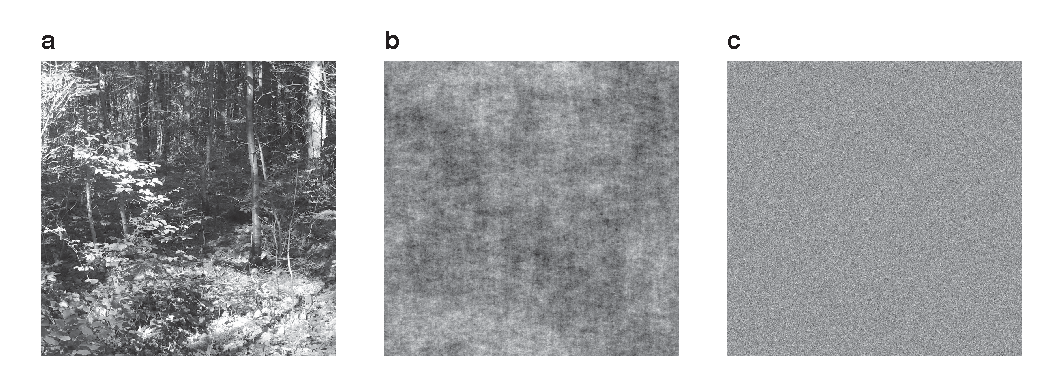
\includegraphics[width=1.025\textwidth]{graphics/figure_images}
    \caption[Natural and artificial images]
    {Comparison of natural and artificial images. \textbf{a} Natural image patch taken from the in-house library used in \citet{Leonhardt:2016ex}. \textbf{b} Same image after randomization of phase. \textbf{c} Same image after additional flattening of the characteristic amplitude spectrum.}
    \label{fig:image}
\end{figure}

This is easily visualized by manipulating pictures in Fourier space \citep{Hyvarinen:2009hf}. Unaltered images exhibit edges, gradients, homogeneous textures, and segregated objects (Figure \ref{fig:image}a). These typical features also extend to natural video sequences. Randomizing the phase structure of images scrambles their higher-order structure and yields phenomenologically atypical textures, even though the manipulation conserves second-order statistics as a consequence of the natural amplitude spectrum (Figure \ref{fig:image}b). Nonetheless, local patches may still resemble real image features. Finally, when one flattens the image's amplitude spectrum, only unambiguously artificial noise remains (Figure \ref{fig:image}c). Critically, at each stage we can clearly distinguish between images that fall within or outside of the distribution of natural visual scenes.

Large corpora of calibrated natural images like the ones generated by \citet{vanHateren:1998jt} or \citet{Tkacik:2011aa} make it possible to characterize fundamental statistical properties. Below, I describe a subset of relevant features, ranging from first-order parameters to more complex traits.

\subsubsection{Luminance}

\begin{figure}
    \centering
    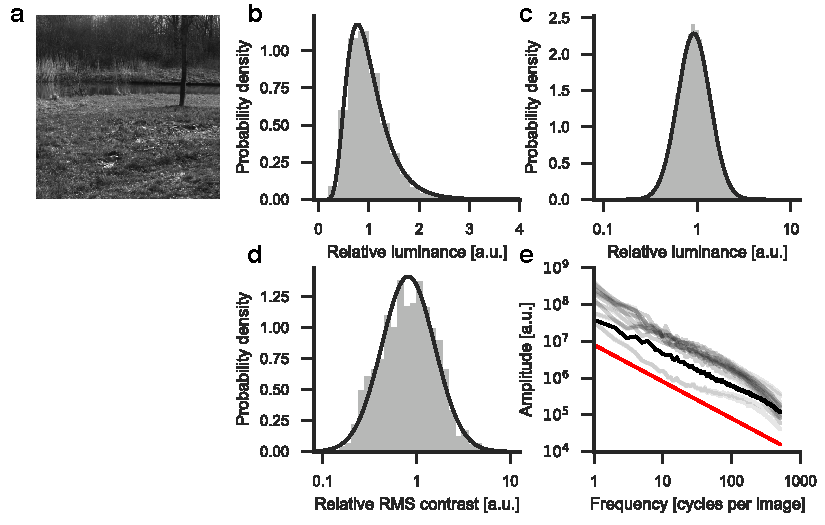
\includegraphics[width=1\textwidth]{graphics/figure_natstats}
    \caption[Fundamental statistics of natural images]
    {Fundamental statistics of natural images. \textbf{a} Calibrated natural image from the database by \citet{vanHateren:1998jt}. \textbf{b} Distribution of per-pixel luminance values for the image in \textbf{a}, normalized to a mean luminance of $1$. The black curve depicts a log-normal fit to the empirical values. \textbf{c} Same distribution replotted on a logarithmic luminance scale. The black curve depicts a corresponding normal distribution fit to the rescaled values. \textbf{d} Distribution of log-scaled local contrast for the image from \textbf{a}. Root-mean-square (RMS) values were calculated as the ratio of standard deviation to mean in patches of size $30 \times 30$ pixels and normalized such that the average contrast is $1$. The black curve shows a log-normal fit to the empirical distribution. \textbf{e} Log-transformed amplitude spectrum of natural images. The image from \textbf{a} is depicted by the black line; grey lines correspond to 20 other images from the same database. The red line shows an arbitrarily scaled function $1/f$ for reference, indicating the typical spatial frequency distribution of natural images.}
    \label{fig:natstats}
\end{figure}

As a first step, one can measure the distribution of pixel luminance (Figure \ref{fig:natstats}a,b). After per-image normalization, linearly scaled luminance values in natural images are typically positively skewed \citep{Laughlin:1981wn,Brady:2000aa,Geisler:2008gu}. That is, pixels that are dark relative to average luminance numerically outweigh bright ones. When put on a logarithmic scale, this results in a symmetric distribution (Figure \ref{fig:natstats}c). The finding applies universally to image sets across a multitude of environments. Presumably, the asymmetry follows from basic physical principles.

\subsubsection{Contrast}
Another fundamental statistic is local contrast. Its quantification is less straightforward than in the case of luminance as it requires assumptions about the sensory system and the stimulus under investigation. Common definitions are the difference between feature and background luminance divided by the latter (Weber contrast), the standard deviation of normalized luminance in a small image patch (root-mean-squared contrast; see Figure \ref{fig:natstats}d), or the difference of luminance extrema normalized by their sum (Michelson contrast, often applied to periodic stimuli like sine gratings). Alternatively, in analogy to processing in retinal ganglion cells, contrast can be modeled as the response of divisively normalized center-surround receptive fields.

Here, a similar asymmetry as for luminance emerges (Figure \ref{fig:natstats}d). At all spatial scales, natural images contain more dark (OFF) than light (ON) contrast \citep{Ratliff:2010kb,Cooper:2015in}. This is a direct consequence of the positively skewed luminance distribution. Moreover, luminance and contrast are not fully independent: their correlation is small but clearly negative \citep{Geisler:2008gu}.

\subsubsection{Spatial patterns}
Spatial structure is one of the most informative aspects of any scene. A hallmark of natural images is the shape of their Fourier amplitude spectra \citep{Geisler:2008gu}. The average contribution of components falls with increasing frequency and is well modelled by the function $1/f^n$ with $n\approx1.0$ \citep{Field:1987ua,Ruderman:1994ty,Dyakova:2015dy}. This is demonstrated in Figure \ref{fig:natstats}e for a range of scenes. As a consequence, natural images are approximately scale-invariant. Zooming in or out does not substantially affect the shape of the Fourier spectrum. Interestingly, the pink noise model also reproduces spatial properties of local patches in naturalistic video sequences \citep{Dong:1995aa} even though the complex statistics of animal movement make the task of gathering ecologically relevant stimuli difficult.

As discussed above, $1/f$ noise serves as a reasonable local approximation to realistic images but falls short in several ways. One of them is the linearly symmetric luminance distribution which does not reproduce natural skew \citep{Geisler:2008gu}. Moreover, it fails to model the heavy-tailed response distribution of arbitrary receptive fields scanning natural scenes \citep{Field:1987ua}. Clearly, the Fourier spectrum does not provide an exhaustive description of real-world spatial features. Natural images show pronounced co-linearity, parallel contours, sharp transitions, and many other forms of spatial regularity that go beyond simplistic lower-order features.

\subsubsection{Other properties}
In addition to the most salient subset of features outlined above, researchers have mapped the natural statistics of many additional visual scenes. These efforts include measurements of depth \citep{Huang:2000aa}, color \citep{Ruderman:1998aa,Wachtler:2001aa}, and optic flow \citep{Roth:2005aa,Roth:2007bg}, but are often limited in throughput by available sensors. Reliable estimation of natural statistics in high-dimensional spaces requires sufficient volumes of data. For this reason, static but large image databases have been an important foundation for research in this space \citep{vanHateren:1998jt}.

\subsubsection{Visual ecology}
To relate any visual system to naturally occurring stimuli, a reasonable approximation of the neuro-ecologically relevant image distribution is required. Available natural scene libraries are biased toward human visual surrounds when it comes to choice of environment, perspective, focal length, resolution, and other parameters \citep{Tkacik:2011aa}. Many of these qualities are at odds with the experience of a typical fruit fly. For instance, the \textit{Drosophila} eye processes scenes at the comparatively low resolution of approximately $25 \times 25$ facets or "pixels", covering close to $180\degree$ of azimuth at a separation of $\approx5\degree$ \citep{Borst:2009gv}. The resolution of the fly eye as well as its spatial acuity are orders of magnitude below that of its human counterpart. Moreover, not much is known about the ground-truth visual statistics of the environment in which \textit{Drosophila} and its precursors evolved.

Spatial discrepancies, however, are attenuated by the aforementioned invariance of realistic image amplitude spectra. Generally, fruit flies are extremely widespread and resilient organisms. Their brains possess comparatively few neurons, resulting in limited degrees of freedom. As a consequence, visual adaptation is unlikely to be deeply environment-specific \citep{Dickinson:2014aa}. Finally, many of the lower-order statistics discussed above appear to be due to fundamental properties of the world and thus generalize to visual environments across the board \citep{Geisler:2008gu,Simoncelli:2001dn}. \citet{vanHateren:1997vg}, for instance, studied fly retinal processing and gathered reasonably natural luminance time series simply by walking through a forest while recording the output of a LED attached at human eye level.

\subsection{Information theory}

Information theory, a branch of probability theory initially developed in the context of electrical communication channels \citep{Shannon:1948aa}, provides powerful techniques for studying neural and particularly sensory processing \citep{Borst:1999hw}.

The activity of visual sensory neurons is generally related to some parameter of a given stimulus. In the case of motion-selective units, this could include direction, velocity, acceleration, or contrast. Classically, experiments probe possible relationships by systematically varying parameters and recording stimulus-response curves to determine what feature of the visual input is encoded. When considering the function of neural circuits, however, precision of encoding also matters: we want to quantify rigorously not just what but also how much stimulus-related information a sensory cell carries. Information theory offers a principled way of studying relationships of this type by measuring the reduction in uncertainty about the stimulus any given neural signal provides.

Formally, this is achieved by determining the entropy $H$ of appropriate distributions and closely related to ideal-observer models of decoding. Consider a simple experiment in which the responses of direction-selective neurons are measured as a function of a specific stimulus feature like pattern velocity. Such measurements are stochastic, so we take stimulus and response to be random variables $S$ and $R$ with associated probability distributions. We can quantify our uncertainty about a variable by calculating the Shannon entropy
\begin{equation}
    H(X) = - \sum_{i} p(x_i) \log_2 p(x_i) \geq 0
\end{equation}
in which $i$ indexes all possible discrete outcomes $x$ of $X$ and $p(x)$ denotes the probability of $x$ occurring \citep{Cover:2006aa}. For the logarithm with base two, entropy is measured in bits.

Intuitively, information rigorously measures how much an ideal observer learns about the stimulus from the neuron's response. This intuition can be made precise by expressing the quantity as a difference between full stimulus entropy and residual entropy after observing the response
\begin{equation}
    I(R; S) = H(S) - H(S|R).
\end{equation}

This quantity is called mutual information between $R$ and $S$ \citep{Cover:2006aa}. From its definition, we can readily see that the measure is either positive if we learn something about the stimulus or exactly zero if knowing the response does not reduce our uncertainty at all (in which case $H(S) = H(S|R)$ holds). The latter occurs whenever $R$ and $S$ are statistically independent, and thus lines up with experimental intuition.

By expanding the expression above, we can calculate the information about a certain stimulus condition $s_x$ provided by the neuron's response $R$ as
\begin{equation}
    I(R; s_x) = \sum_{i} p(r_i | s_x) \log_2 \frac{p(r_i | s_x)}{p(r_i)}
\end{equation}
where $i$ indexes the set of all enumerated responses, $p(r_i)$ denotes the marginal probability of a specific response across all stimulus conditions, and $p(r_i | s_x)$ denotes the response probability conditioned on a specific stimulus \citep{Borst:1999hw}. Average information for the full stimulus set is then computed as the probability-weighted sum of specific per-stimulus information
\begin{equation}
    I(R; S) = \sum_{j} p(s_j) I(R, s_j)
\end{equation}
where $j$ indexes stimuli. This comes out as the mean if stimuli are equally probable (as is the case in balanced experimental designs). Note that information as defined here critically depends on decisions like response binning and the choice of stimulus conditions. In a sense, values hinge on the choice of alphabet used to represent the experiment.

For some designs, one can derive theoretical bounds on the transmission capacity of neural channels and estimate normative qualities like the efficiency of a neural code by weighing transmitted information against maximally possible response entropy. It also extends naturally to the encoding of dynamic stimuli. Note that information theory is a universal method. It works in the absence of a specific response model and without making strong assumptions about the function of a sensory system or the constraints under which it operates.

The technique has been used to quantify information rates, coding efficiency, and transmission bounds for several model systems including motion-sensitive neurons in flies \citep{Bialek:1991aa,vanSteveninck:1997aa,Haag:1998wr,Weber:2012dr}, electroreceptors in fish \citep{Wessel:1996aa}, and retinal ganglion cells in the salamander \citep{Warland:1997aa}. Remarkably, measured information rates depend on the choice of stimulus ensemble. In frog auditory neurons, for instance, \citet{Rieke:1995aa} found efficiency values close to \SI{90}{\percent} when they tested naturalistic input.

\subsection{Efficient coding}
Sensory systems evolve under a multitude of constraints \citep{Sterling:2015aa}. One of them is the need to detect stimuli that are survival-critical. Another is the need to perform this task using a minimum of metabolic energy. A third comes from the natural distribution of environmental features. The efficient coding hypothesis, going back to \citet{Attneave:1954aa}, \citet{Barlow:1961aa}, and others, formalizes this approach to understanding biological sensors. Their theory was of course heavily influenced by the development of information theory which made a rigorous quantification of notions like channel capacity and redundancy feasible.

Efficient coding assumes that the goal of a sensory system is to represent as much relevant information as possible using the smallest feasible amount of resources. Selecting appropriate objective functions is, of course, fraught with difficulty. Ground truth constraints are generally not available and sensory organs often support a broad range of behavioral functions, each of which may necessitate a different definition of relevance. Nonetheless, the theory has successfully predicted features of real systems by assuming basic, tractable goals. In the sensory periphery, this usually takes the form of general preservation of information, thus maximizing the number of possible downstream use cases.

The main target of early vision then becomes reduction of redundancy. Ideally, signals carried by peripheral sensory neurons should be statistically independent in order to minimize wasteful duplication of information. Natural images exhibit regular statistics such as characteristically shaped power spectra that give rise to specific correlation structures. By removing such correlations and emphasizing deviations from expected natural statistics, an operation commonly termed whitening, early vision minimizes energy expenditure while conserving features of the stimulus that are presumed to be behaviorally relevant.

\begin{figure}
    \centering
    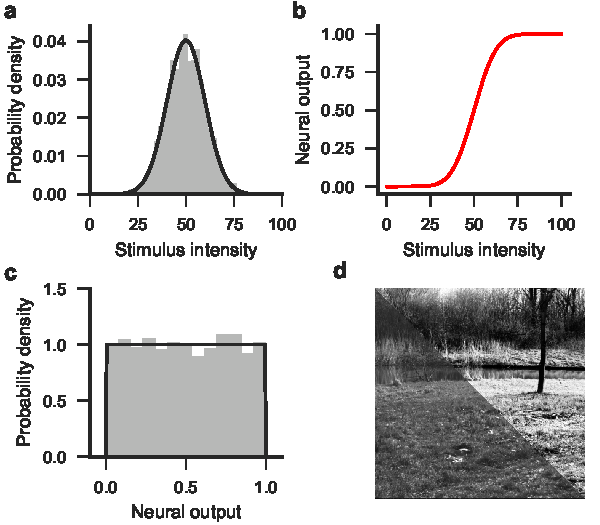
\includegraphics[width=1\textwidth]{graphics/figure_equalization}
    \caption[Histogram equalization]
    {Histogram equalization as a demonstration for efficient coding of sensory stimuli. \textbf{a} Sensory samples drawn from a Gaussian stimulus distribution (black line; $\mu = 50, \sigma = 10$). \textbf{b} Neural transfer function. If this approximates the cumulative distribution function of the stimulus-generating process (as is the case here), the resulting output histogram is effectively normalized. \textbf{c} Distribution of samples in \textbf{a} transformed by the function depicted in \textbf{b}. The black line is a uniform distribution fit to the empirical values. \textbf{d} Histogram normalization as a contrast-enhancing technique. The lower triangle shows a picture as taken from the database by \citet{vanHateren:1998jt}; the upper triangle shows the result of equalizing the luminance histogram.}
    \label{fig:equalization}
\end{figure}

Work on the fly visual system provides seminal demonstrations of this principle at work. \citet{Laughlin:1981wn} measured naturally occurring luminance distributions and compared the resulting histograms to corresponding response functions of lamina monopolar cells which form the first processing stage after the light-sensitive photoreceptor. In line with predictions from efficient coding, these response functions effectively equalized the input histograms, making all outputs equally likely under the assumption of a natural stimulus distribution. A related study \citep{Srinivasan:1982uq} could show that lateral inhibition in the fly retina reliably removes the long-range correlations typical for natural images, effectively suppressing background, retaining sensitivity to small fluctuations, and implementing a type of predictive coding.

Constraint triples of this type---minimization of resources, maximization of transmitted information, and assumption of some naturalistic stimulus distribution---have also been applied fruitfully to early processing in mammalian systems. Center-surround receptive fields in both retina and lateral geniculate nucleus (LGN) of the cat have been suggested to implement spatial filters that are well suited to whitening the typical power spectra of natural images \citep{vanHateren:1992aa,Atick:1992aa,vanHateren:1993aa}. \citet{Dan:1996aa} confirmed this prediction experimentally by recording LGN responses to natural movies, finding them to be largely statistically independent. \citet{Ratliff:2010kb} argue that the asymmetry between ON and OFF contrast mentioned above explains the difference in numbers between ON and OFF retinal ganglion cells in the vertebrate retina. Interestingly, evidence from primary sensory neurons in V1 of awake mice indicates that adaptation to natural scene statistics partially depends on experience; if the animals are raised in stimulus-deprived environments, predictive coding of specifically real images is abolished \citep{Pecka:2014aa}.

A closely related normative doctrine is that of sparse and distributed coding: the idea that sensory systems like visual cortex aim to represent natural stimuli using a minimum of active neurons \citep{Simoncelli:2001dn}. \citet{Ohlshausen:1996aa}, for instance, optimized a linear generative model to reconstruct natural images under the constraint of activation sparseness. The resulting filters bear a striking resemblance to localized oriented bandpass receptive fields in area V1, indicating that early visual cortex is adapted to the task of efficiently representing real-world stimulus distributions \citep[for a related method based on independent component analysis, see][]{vanHateren:1998jt,Bell:1997ve}.

\subsection{Task-centric approaches}
Efficient coding theory sidesteps the question of task relevance and presupposes that peripheral sensory systems perform lossless compression while maximizing efficiency. This has been a frequent source of criticism \citep{Simoncelli:2003aa}. After all, brains solve particular problems, so not all information is equal. Relevance may well depend on the particular nature of downstream processing or even behavioral state. For this reason alone, efficient coding is unlikely to scale to higher-level computation.

Instead of choosing a generic normative aim like information preservation, one may be able to do better by picking a specific, task-bound objective function. Encouraging examples come from recent advances in artificial pattern recognition \citep{Bishop:2006aa} and specifically the hierarchical models used in so-called deep learning \citep{Goodfellow:2016aa}. Response properties along the visual cortical pathway go from simple local receptive fields in V1 to object-specific and invariant representations in higher areas \citep{Felleman:1991aa,Yamins:2016hg}. Such neurons are sensitive to, for instance, images of cars regardless of perspective or brand. Hierarchical neural networks that mimic aspects of this organization \citep{Fukushima:1980ve} have reached human-like performance on large object recognition data sets, made possible by advances in optimization techniques \citep{LeCun:1989aa} and raw processing power \citep{LeCun:2015dt}. \citet{Yamins:2014gi} modeled an artificial deep network after the primate object recognition cascade consisting of areas V1, V2, V4, and IT. After training this system to recognize classes of objects in natural images, they compared learned weights with representations in the biological system and found striking similarities, at least in higher layers \citep{Cadieu:2014in}. More generally, early stages of visually trained deep networks often exhibit receptive fields that resemble those found in the vertebrate retina or V1 \citep{Yamins:2016hg}.

In psychophysics, studies have successfully predicted texture salience from statistical properties of natural images \citep{Tkacik:2010aa,Hermundstad:2014aa}. By determining maximally informative features in real stimuli, it was possible to predict behavioral performance for a given synthetic texture.

Task-driven approaches have also been applied to the visual system of the fly. \citet{Clark:2014aa} optimized a motion detector to maximize the linear correlation between time-averaged model output and true velocity of rigidly translating natural images. While functionally plausible, this makes strong assumptions about the true goal of motion-sensing elements and evolutionary pressures at work. Other studies put the fly optomotor response in its functional context by evaluating course stabilization in closed-loop, which is the supposed functional target for wide-field motion responses \citep{Warzecha:1996bm,Warzecha:1998tn}. However, this work did not take the natural stimulus distribution into account but used artificial stimuli instead.

Combining behaviorally relevant targets with biologically plausible models appears to be a promising tool for understanding neural computation beyond the sensory periphery. Of course, for complex and highly multiplexed information processing systems like the brain, ascribing goals remains challenging: one may well be wrong about what any given circuit is in fact trying to achieve. Additionally, the approach critically depends on the choice of model---say, a feedforward network for cortical processing as opposed to a more plausible recurrent design---and the techniques used for post-hoc comparisons between model and neural circuit \citep{Yamins:2016hg}.

%%%

\section{Visually guided behaviors in the fly}
Flies and specifically \textit{D.\ melanogaster} exhibit a largely stereotyped, well characterized repertoire of visually driven behaviors \citep{Borst:2014kl}. This has greatly contributed to their ongoing popularity in the field of motion vision. Reflexive responses facilitate the precise measurement of sensory input-output relationships in large volumes. Systems neuroscience derives predictions about neural processing from quantitative descriptions of behavior which drive physiological work. In turn, behavioral tasks provide powerful high-throughput test beds for hypotheses generated from physiological mapping of neural circuits.

A vast majority of behaviors is not explored in the ecological context of freely moving animals but under strictly controlled conditions instead. Deviations from naturalness include head-fixation, tethering, artificial visual stimulation, and synthetic stimulus statistics. Experimental abstraction allows for full control of sensory input and exact observation of fly movements. However, it also runs the risk of mapping artificial behavioral motifs that do not generalize to ecological settings \citep{Krakauer:2017aa}. The controlled approach and in particular the reliable optomotor response have nonetheless shed significant light on the inner workings of motion detection circuitry in flies.

Behavioral assays were a critical component of my work in the studies that comprise the thesis at hand. In the following section, I survey the range of visual reflexes with a clear focus on \textit{Drosophila}, referring to other commonly employed dipteran species (like \textit{Musca domestica} or \textit{Calliphora vicina}) where instructive.

\subsection{Optomotor response}
Flies follow the visual motion of their surround. When for instance tethered to the center of a rotating textured drum, they reflexively attempt to steer in the same direction. This behavioral pattern is termed optomotor response and was a popular model behavior even in early sensory \textit{Drosophila} ethology \citep{Hecht:1934aa,Kalmus:1943aa}.

\begin{figure}
    \centering
    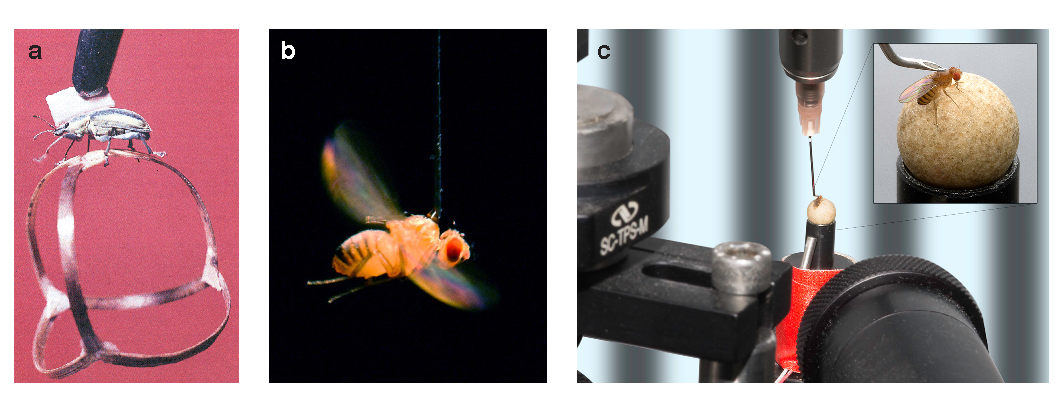
\includegraphics[width=1\textwidth]{graphics/figure_setups}
    \caption[Behavioral set-ups for sensory neuroscience]
    {Quantitative behavioral assays. \textbf{a} The beetle \textit{Chlorophanus} walking on a Y-maze globe in groundbreaking experiments on the insect optomotor response. Image modified from \citet{Hassenstein:1991aa}. \textbf{b} A tethered flying \textit{Drosophila} whose wingbeats are monitored optically. Photo courtesy of the National Science Foundation. \textbf{c} Fruit fly walking on one of the closed-loop treadmill set-ups used throughout this thesis. Surrounding screens project stimuli. Photo by R.\ Schorner.}
    \label{fig:setups}
\end{figure}

A seminal quantitative investigation of the response was conducted by \citet{Hassenstein:1956fa}. They placed \textit{Chlorophanus viridis} on a spherical Y-maze that was light enough to be held and moved by the beetle (Figure \ref{fig:setups}a). This simulated walking while keeping the animal fixed in relation to the visual stimulus. Then, by counting leftward versus rightward choices as a function of various parameters of a rotating drum, they were able to estimate turning tendency in a graded fashion. Their quantitative findings formed the foundation of the algorithmic Hassenstein-Reichardt model for insect optomotor behavior \citep{Reichardt:1961aa} which is discussed in more detail below.

The optomotor response is not exclusive to one mode of fly locomotion \citep{Fermi:1963aa,Gotz:1964bj,Goetz:1973aa,Buchner:1976kd,Goetz:1987aa}. It can be demonstrated in tethered flying \textit{Drosophila} using a torque meter or the difference between wing beat frequencies as a read-out of turning tendency (Figure \ref{fig:setups}b). Moreover, it has been studied in flies walking on treadmill systems that mimic moving ground while keeping the animal in place (Figure \ref{fig:setups}c). While commonly elicited by yaw motion revolving around the vertical body axis of the fly, it generalizes to pitch and roll \citep{Blondeau:1982hd}. When the fly's head is left unrestrained, its movements also track stimulus direction \citep{Hengstenberg:1988kg}.

A plethora of studies has mapped stimulus-dependencies of the optomotor response \citep[see][]{Borst:2010fk}. Critically, the behavior is not driven by the true rotational velocity of the visual pattern. Instead, many other stimulus features influence response magnitude. The most salient properties can be summarized as follows:

\begin{enumerate}
    \item Flies turn in the same direction as the pattern.
    \item Stimulus geometry has a strong effect on the velocity tuning. For sine gratings, increasing the pattern wavelength $\lambda$ shifts the curve towards larger velocities $v$. Critically, the fly optomotor response is tuned not to stimulus velocity but to contrast frequency instead, which for periodic patterns is given by $f = \frac{v}{\lambda}$.
    \item Responses are ambiguous with regard to frequency and only proportional in a limited range. They initially grow with temporal frequency but show a clear optimum after which turning decreases again. In \textit{Drosophila}, measurements of this peak frequency exhibit significant variability but are in the range of \SIrange{3}{10}{\hertz} \citep{Goetz:1973aa,Duistermars:2007aa}.
    \item Optomotor responses are subject to spatial aliasing. If $\lambda$ drops below the Nyquist limit of twice the receptor distance, the response inverts due to undersampling of the sine grating. From this, one can estimate the \textit{Drosophila} sampling base as $\approx \SI{4.6}{\degree}$ of visual space, which matches average inter-ommatidial distance well \citep{Gotz:1964bj}.
    \item The magnitude of the response increases with stimulus contrast.
\end{enumerate}

Functionally, the reflex is usually interpreted as a compensatory steering mechanism \citep{Gotz:1968aa,Heisenberg:1984aa}. Flies are capable of long-duration flight in adverse surroundings \citep{Goetz:1987aa,Dickinson:2014aa}. They also perform acrobatic maneuvers whose instantaneous rotational velocity may well exceed \SI{2000}{\degree\per\second} during unrestrained flight, all at forward speeds that can reach \SI{1.0}{\metre\per\second} \citep{Land:1974dp,Mronz:2008eb,Censi:2013cya}. At the same time, the weight of an individual fruit fly is on the order of \SI{0.2}{\milli\gram} \citep{Seiger:1966a}. This makes them preciously vulnerable to external perturbations like sudden gusts of wind. Internal sources of noise, like small asymmetries in wing morphology, add to the problem.

In concert with proprioceptive mechanisms, the optomotor response confers some protection against unintended path deviations. Any turning response that is syndirectional with global optic flow will eventually return the fly to straight heading, assuming that the estimated optic flow provides an accurate read-out of ego-motion. The optomotor response implements a simple, reflexive feedback system that keeps the fly on course\footnote{Note that some studies have suggested that \textit{Drosophila} is capable of modulating the strength and even sign of optomotor orientation behavior through stochastic adjustment and subsequent evaluation of visual feedback \citep{Wolf:1986ii,Wolf:1992aa}.} \citep{Borst:2014kl}. In this vein, some authors have argued that the non-monotonous velocity tuning of the motion sensor keeps the system from falling into irrecoverable oscillations \citep{Warzecha:1996bm}. Comparable locomotor reflexes are found in other insects or fish \citep{Arnold:1974aa,Portugues:2009aa} and the optomotor response closely resembles the optokinetic nystagmus that stabilizes the eye during movement \citep{Buttner:2007aa}.

Traditionally, optomotor responses have been studied in tethered animals. If the functional logic outlined above holds, then it should also be possible to observe a visually induced following reflex in unrestrained behavior. Counter-intuitively, \citet{Goetz:1970aa} found that groups of unrestrained fruit flies placed in a rotating drum moved against the direction of the wall pattern. This was later successfully explained as a consequence of complex superpositions of external stimulus and self-induced translating optic flow \citep{Goetz:1975aa}. \citet{Strauss:1997ut} used on-line tracking and live generation of appropriate stimuli to suppress self-generated feedback and confirmed tethered turning behavior in free walking. While tracking flying flies in a large arena, \citet{Mronz:2008eb} could elicit prolonged curved trajectories and largely suppress the body saccades typical for \textit{Drosophila} flight by rotating the cylinder's texture.

\subsection{Landing and escape response}
Flies are notoriously competent at evading fast-moving objects and rarely collide with static landmarks. Motion sensors signal imminent collisions through particular patterns of translational optic flow. Approaching a textured surface results in visual expansion whose magnitude correlates with distance and thus, critically, time to impact \citep{Koenderink:1986um}. By selectively extracting looming flow fields, flies can trigger an appropriate response. When at rest, they initiate a fast and largely stereotyped escape maneuver. When flying, they either evade or perform the wing and leg adjustments required for safe landing \citep{Borst:2014kl}.

Several studies have investigated the latter condition in tethered experimental settings. When stimulated with laterally expanding square-wave gratings, \textit{Drosophila} robustly steer away from the focus of expansion \citep{Tammero:2002aa}. Centered expansion, on the other hand, activates a landing sequence. \citet{Duistermars:2007aa} systematically compared the tuning properties of expansion-triggered evasion and rotation-triggered optomotor response. The two pathways differed in pooling and contrast sensitivity, yet, aspects like temporal and spatial sensitivity were preserved. This indicates that both behaviors draw from the same set of motion-sensitive units which are then processed differently.

Centrally positioned expansion of sine or square-wave gratings prompts the landing response which consists of a fixed sequence of postural and steering-related adjustments \citep{Goodman:1960aa,Braitenberg:1966aa,Borst:1986wx}. Critically, the delay leading up to initiation of this program depends on spatial and temporal aspects of the expanding stimulus. By manipulating these parameters, \citet{Bahde:1986eh} demonstrated that a single set of motion detecting units could feasibly underlie both optomotor and landing response in the housefly \textit{M.\ domestica}. Their model simply integrates motion signals up to a certain threshold after which the landing sequence is started. This system was capable of reliably predicting response latencies.

When at rest, flies respond to fast expansion by rapidly initiating a controlled jump. This happens within $\approx\SI{200}{\milli\second}$ of stimulus onset and is not completely stereotyped. In a majority of cases, flies manage to coordinate their take-off such that they escape away from the looming stimulus, which hints at a surprisingly elaborate transformation from visual input to motor output \citep{Card:2008aa}. Recent high-resolution tracking of escape responses revealed a subtly bimodal distribution of time courses, indicating two distinct, stimulus-dependent escape programs and thus even more complex behavioral phenomenology \citep{Reyn:2014aa}. Intriguingly, \citet{Muijres:2014aa} tracked the flight kinematics of looming-triggered escape responses in freely flying \textit{D.\ melanogaster} and observed extremely rapid banked turns consisting of carefully calibrated directional shifts and counter-shifts. This survival-critical sequence is completed within a small number of wing beats and testament to the impressive maneuverability of fruit flies.

\subsection{Beyond optic flow}
All behaviors discussed so far were derived from global optic flow. Of course, the visual environment of the fruit fly provides cues beyond wide-field motion.

A prominent example among behaviors driven by other stimuli is fixation. Ego-motion results in the largely coherent flow that spans the complete visual field and drives the optomotor response. Superimposed onto this motion background are the relative movements of nearby objects. Flies need to track such entities in order to avoid predators, find conspecifics, and navigate between landmarks.

This can be studied experimentally. Depending on the separation of two bars projected onto the wall of an arena, walking flies either track the area between the two stripes or choose one of two as they become more distant \citep{Horn:1975aa}. \citet{Maimon:2008go} studied fixation behavior in freely flying \textit{Drosophila} and discovered a remarkable trade-off between approach and avoidance by varying the height of a rod placed in an arena. When the bar was long, flies would approach and circle it. When it was shortened, the bar became aversive; flies now tended to steer clear of the object. The pattern is reminiscent of a famous behavioral setting, Buridan's paradigm\footnote{The set-up is aptly named after a thought experiment attributed to the French priest and philosopher Jean Buridan. In it, an equally hungry and thirsty donkey is trapped between food and water and eventually starves to death \citep{Knowles}.} \citep{Buelthoff:1982aa}. In a behavioral chamber with two vertical rods, flies will ceaselessly walk from one to the other, entering a seemingly inescapable loop of fixation and anti-fixation.

Experiments in tethered flies have illuminated some functional aspects of the fixation response. \citet{Reichardt:1969aa} coupled the output of a torque meter to the position of a vertically elongated bar which enabled the fly to control its visual input in a semi-realistic closed-loop setting. Interestingly, \textit{M.\ domestica} kept the target in an on average frontal position. \citet{Reichardt:1973aa} ascribed this behavior to asymmetric motion responses. In an open-loop setting, a black stripe moving from front to back resulted in a stronger optomotor response than its back-to-front counterpart. In closed-loop, this imbalance would eventually push the stripe toward the front. In later theoretical treatments of fixation and orienting behavior, the imbalance was analyzed as the superposition of a optomotor-like response and the response of a position system that determines the position of a salient cue and orients the fly towards it \citep{Poggio:1973aa}. Similarly, \citet{Pick:1974aa} argued that flies simply orient towards flicker. Recent work used neurogenetic silencing techniques to isolate motion- from position-driven responses and found evidence for a position system of the predicted type in \textit{D.\ melanogaster} \citep{Bahl:2013ha}. Interestingly, the visually guided orientation behavior of fruit flies goes well beyond reflexes. \citet{Ofstad:2011aa}, for example, reported robust associative learning based on visual landmarks.

Fruit flies exhibit various other visual behaviors. \citet{Bahl:2015cqa} have recently provided evidence that \textit{Drosophila} respond robustly to temporally modulated spatial contrast. The functional significance of this sensitivity, however, remains unclear. In an early piece of sensory ethology, \citet{Carpenter:1905aa} described the tendency to approach light in a fruit fly species. This is an example of phototaxis, one of the most simplistic visual reflexes in the animal kingdom.

On the more sophisticated end of the spectrum, studies have shown that fruit flies utilize the polarization of light to orient their course \citep{Weir:2012aa}. Polarized light results from atmospheric scattering as well as certain reflecting surfaces and provides critical navigational cues. The information is mediated by two physiological pathways, one sensitive to dorsal polarization emanating from the sky and the other to ventral reflectance-derived stimuli \citep{Wernet:2012aa}. The system may explain the reported long-term navigation feats of certain \textit{Drosophila} species which have been reported to travel up to $\SI{10}{\kilo\metre}$ in the desert \citep{Dickinson:2014aa}.

Finally, fruit flies possess a limited repertoire of color-mediated behaviors \citep{Menne:1977aa}. However, this is limited to spatially coarse types of visual sensing. For instance, flies learn to differentiate green and blue in an aversive association task \citep{Schnaitmann:2013aa}. The optomotor response, on the other hand, operates with luminance information only. If a square-wave grating consists of differently colored but brightness-matched stripes, no turning is elicited \citep{Yamaguchi:2008aa}.

\section{Stimulus design}
A key step toward understanding sensory systems is the measurement of input-output relationships. In the case of the visual apparatus, this takes the form of displaying controlled, parameterized visual patterns and then quantifying responses at various levels of the processing cascade. Typically, the relevant outputs are neural or behavioral activity. As with any system, the choice of stimulus determines what we can learn about the transformations accomplished. Below, I review common classes of motion stimuli used in the investigation of the fly optomotor response.

\subsection{System identification techniques}
As discussed above, the statistics of natural optic flow are complex and hard to control in experimental contexts. Instead of reverse-engineering the function of a visual system from the top down, it appears preferable to use simplified stimuli and explore relevant computations from the bottom up. The engineering sub-field of signal processing offers a multitude of principled tools that support the rigorous identification of systems based on such input-output measurements.

Oriented moving sine gratings are the workhorse of motion vision research. They can be fully specified using a small number of parameters: spatial wavelength $\lambda$, velocity $v$, mean luminance $I$, contrast $\Delta I$, and if required the angle of orientation in two-dimensional space. Conveniently, when sampled at a single location, the resulting temporal signal is again a sinusoid with contrast frequency $f = \frac{v}{\lambda}$. Neighboring signals are modulated at the same frequency but differ in relative phase. This means that the brightness input to the photoreceptors has clearly defined mathematical properties, rendering them amenable to the rigorous tools of Fourier analysis and filter theory. Examples of this approach include \citet{Gotz:1964bj}, who estimated the sampling base of local motion detectors in the fruit fly via quantification of spatial aliasing, or \citet{Egelhaaf:1989wf}, who employed spectral analysis to characterize the non-linearity underlying motion computation in the blowfly \textit{C.\ erythrocephala}. In practice, true sinusoidal stimuli are often replaced by periodic square-wave gratings whose Fourier expansion consists of all odd-integer harmonics of some fundamental spatial frequency $\lambda^{-1}$. Such stripe patterns are easier to construct in experimental settings and result in similar temporal photoreceptor signals if substantial spatial blurring is assumed. Moving sinusoidal gratings can be stacked and blended to produce stimuli of higher complexity. A famous example are so-called plaids which consist of two angled moving gratings and may produce ambiguous motion percepts \citep{Adelson:1982aa}. As a special case, counterphase flicker can be constructed from identically oriented gratings drifting in exactly opposite directions and has been used fruitfully in fly vision research \citep{Bahl:2015cqa}.

Filter theory provides another high-throughput tool for system identification in the form of white-noise techniques and its close relatives \citep{Dayan:2001aa}. Instead of mapping the relationship between a parameter of, say, a sinusoidal motion stimulus and its associated response one by one, we can feed dynamic input into the system and recover the transfer function by means of reverse-correlation. This works efficiently if the distribution of the relevant parameter is as decorrelated as possible; in case of a motion stimulus, for instance, the spectrum of velocities ought to be close to flat. The properties of the resulting kernel may then offer insight into the inner workings of the motion detection system. This class of stimuli has been successfully applied to walking behavior in fruit flies \citep{Theobald:2010dt,Aptekar:2013iv} as well as response properties of motion-sensitive cells in the fly visual system \citep{Borst:2005dr,Weber:2010ic}.

Finally, traveling edges offer yet another tool for motion research. They combine relatively simple stimulus statistics with polarity-specificity; that is, they are defined purely by one direction of luminance change (ON or OFF). This pattern class has had substantial impact on the field of motion vision, particularly in the fruit fly \citep{Joesch:2010fw,Eichner:2011ic,Clark:2011gw}.

\subsection{Visual illusions}
The use of visual illusions can be traced back to the earliest roots of psychophysics, with a vague description of motion aftereffects appearing in Aristotle's \textit{Parva Naturalia}. Illusory stimuli elicit naturalistic impressions of motion in the absence of actual physical movement. The fundamental logic then runs as follows: While multiple algorithms may be able to explain the standard phenomenology of motion vision, studying edge cases and deviations from intended function could feasibly narrow down the set of compatible mechanisms.

A classical illustration of this psychophysical principle is the apparent motion percept elicited by two adjacent light spots flashing in quick temporal succession, so-called phi motion \citep{Wertheimer:1912aa}. The immediacy of the percept critically depends on both spatial and temporal separation; if both are chosen correctly, the two events combine to produce the vivid impression of movement. This stimulus has been extended to whole patterns \citep{Anstis:1970tv} and is closely related to the beta motion illusion that underlies the perceptual fluidity of discretized video sequences. In the study of insect motion vision, there is a rich history of using apparent motion to elucidate sensory mechanisms as it allows the isolation of a minimal localized event with clearly defined spatiotemporal parameters. The reverse-phi phenomenon in particular has substantially influenced the design of detector models. If apparent motion is accompanied by a contrast reversal of the pattern, perceived direction tends to invert \citep{Anstis:1975tu,Chubb:1989tw}. This effect is not limited to human perception. Many visual systems across the animal kingdom are subject to the illusion, including the fly \citep{Egelhaaf:1992wh,Orger:2000cy,Krekelberg:2005cb,Tuthill:2011ic,Eichner:2011ic,Clark:2011gw}. The observation was a critical factor in the development of correlation-based motion detectors \citep{Hassenstein:1956fa}.

Most research on insect vision is concerned with first-order or Fourier motion which is defined by pairwise spatiotemporal correlation of luminance. In this scheme, both phi and reverse-phi stimuli find a convenient explanation as positive and negative correlation, respectively. Physical motion induced by displacement of objects or ego-motion generally produces such dependencies. Psychophysical experiments, however, provide ample evidence for sensitivity to higher-order correlations \citep{Lu:2001vf}. Using an optomotor stimulus in which motion was defined by local contrast reversal within a random stripe pattern, \citet{Theobald:2008et} elicited optomotor responses to second-order motion in tethered flying \textit{Drosophila}. \citet{Hu:2010gx} developed a novel class of stimulus to probe higher-order motion, so-called glider patterns. Here, a deterministic set of update rules seeded with random black and white pixels produces stochastic displays whose average correlation structure is limited to one particular spatiotemporal order. Phi and reverse-phi are recovered as the edge case of two-point correlation, but the algorithm naturally extends to three- and four-point stimuli. Using this scheme, \citet{Clark:2014aa} could demonstrate that walking fruit flies robustly respond to correlations defined by three points in space and time.

\subsection{Naturalistic stimuli}
As discussed in previous sections, naturalistic stimuli represent a double-edged sword. Sensory systems are evolved in particular environments and for particular tasks, so using ecologically plausible stimuli may help illuminate the inner workings of the fly visual system. This advantage comes at the cost of not being able to clearly relate stimulus features to particular aspects of the response.

Several investigations of fly motion vision have attempted to strike a compromise between the two extremes. \citet{Wertz:2009hb}, for instance, studied binocular integration of optic flow using simulated rotations around various body axes in a virtual three-dimensional room whose walls were lined with checkerboard textures. The visual statistics of this stimulus are simpler than they would be in nature, but the motion pattern resembles reality more than a traveling grating would. In a complementary approach, several studies have used natural textures such as panoramic images of real environments to examine response properties of motion-sensitive units in the fly visual system \citep{Straw:2008hh,OCarroll:2011gj}. Here, synthetic motion kinetics were traded off against a more reasonable approximation of natural image statistics. \citet{Lewen:2001tz} took this approach one step further by mounting \textit{Calliphora} on a mobile platform that allowed electrophysiological recordings from motion-sensitive cells while the fly rotated in a wooden area. This way, they were able to guarantee that dynamic range and general statistics of the stimulus are truly natural.

%%%

\section{Tools for circuit neuroscience}
Progress in neuroscience is often driven by advancement of the technologies we use to study circuits. Some of the earliest breakthroughs in neural physiology heavily depended on the development of novel measurement devices. For instance, it was the Lippmann electrometer that allowed Edgar Adrian to measure minuscule currents in the toad optic nerve. His observations lead to the Nobel Prize-winning discovery that cells in the retina respond electrically to visual changes \citep{Adrian:1928aa}.

Due to its long-standing history in the field of genetics, \textit{D. melanogaster} offers the arguably richest toolkit for monitoring and manipulating neurons among the dominant model organisms in neuroscience, fruit fly, mouse, nematode, and zebrafish \citep{Venken:2011hf}. In the subsequent sections, I review some of the most prevalent techniques in the field of fruit fly neuroscience.

\subsection{Neurogenetics}

An overarching goal of sensory neuroscience is to relate particular functions to particular neurons or groups thereof. Often, this is achieved by altering or disrupting neural function and then assaying neural and behavioral defects.

\subsubsection{Mutagenesis}
Classically, such dependencies have been established via gene-centric approaches. This often involves mutagenic disruption of stochastically selected genes and subsequent screens for specific phenotypes, the so-called forward direction from phenotypes of interest to involved genes. Reverse screens start from specific genes and then map phenotypic outcomes. Groundwork for this approach was laid by Thomas Hunt Morgan whose serendipitous discovery of the \textit{white} mutation and its consequence, a distinct lack of eye pigmentation, critically illuminated hereditary mechanisms in the fruit fly \citep{Morgan:1910aa}. Within visual neuroscience, one may be able to assign function to certain brain areas by carefully correlating mutation-induced changes in neural structure with behavioral effects.

A paradigmatic and germane example comes from \citet{Benzer:1967aa} who screened fruit flies in a phototaxis task while efficiently creating mutations through application of ethylmethane sulfonate. The principle behind his behavioral set-up was modeled after the chemistry technique of countercurrent distribution, which allowed for high-throughput fractionation of visual phenotypes. \citet{Gotz:1964bj} investigated the optomotor behavior of \textit{white} mutants and found specific deviations from wild-type behavior which could be explained from a lack of shielding pigment. The population fractionation approach was later successfully extended to optomotor behavior \citep{Goetz:1970aa}. Importantly, post-hoc evaluations of neural aberrations in the optic lobe later allowed some limited inference about causal relationships between neural substrate and visual function \citep{Pak:1970aa,Heisenberg:1975aa,Heisenberg:1978aa,Fischbach:1981aa}.

\subsubsection{Binary expression systems}
Disruption of gene activity is likely to affect brain function widely and indiscriminately which puts inherent limits on the usefulness of mutagenic approaches in circuit neuroscience. To draw clear and causal conclusions about neural function, one needs to be able to flexibly manipulate groups of cells with high precision in space and time. This is generally accomplished through the use of binary expression systems like GAL4-UAS \citep{Venken:2011hf}.

Such systems consist of two components: a driver or transactivator that determines \textit{where} expression occurs and a responder that determines \textit{what} is expressed. GAL4 is a yeast-derived transcriptional activator protein that binds specifically to a class of regulatory sites called upstream activating sequences (UAS). Upon binding, the transcription of a chosen responder is initiated. \citet{Rubin:1982aa} pioneered the use of transposable P-elements to stochastically and stably insert DNA sequences into the fly genome. Using this technique, \citet{Brand:1993vw} could place the transgene coding for GAL4 under the control of random endogenous enhancers. Depending on the specific locus, GAL4 is expressed in different subsets of cells. This provides the desired specificity. Analogously, one can insert a combination of UAS and desired effector gene into the genome of another fly line. Assuming that no critical locus is affected, both driver and responder strains are healthy. In isolation, neither GAL4 nor the activating sequence have adverse effects. Critically, the effector gene is not transcribed in the absence of binding GAL4.

If a driver strain shows a relevant expression pattern, it is easily crossed to a chosen effector line. In the resulting progeny, the effector is then transcribed ectopically only in GAL4-labeled cells. This powerful technique thus makes it possible to express virtually arbitrary transgenes in selected groups of neurons. Concerted research effort has since greatly enhanced the technique, improving expression levels as well as rendering the method more reliable \citep{Pfeiffer:2010aa,Pfeiffer:2012bu}, and has produced massive libraries of GAL4 lines with anatomically well-characterized expression patterns \citep{Pfeiffer:2008aa,Jenett:2012aa,Kvon:2014aa}.

Standard GAL4 lines are not always sufficiently specific to one neuronal type or even group of types. Intersectional strategies offer a simple algebra for refining expression patterns. The simplest operation is the addition of multiple GAL4 lines. Conversely, yet another yeast-derived protein, GAL80, can act as a repressor of GAL4; GAL80-expressing cells are thus subtracted from the original GAL4 pattern \citep{Lee:1999aa}. Variants of GAL80 whose efficacy depends on temperature offer temporal control over this process, which has proven useful in pausing GAL4-driven expression during critical developmental periods \citep{McGuire:2003aa}.

A particularly powerful operation is provided by the split-GAL4 system \citep{Luan:2006aa}. GAL4 can be divided into its two constituents, the activation domain GAL4-AD and the DNA binding domain GAL4-DBD. By putting the two hemidrivers under the control of separate regulators, their simultaneous expression is restricted to the intersection of the two. Only where both are present do the two parts then recombine and become effective at binding to UAS. This adds logical conjunction to the set of available operations. split-GAL4 lines have proven especially useful in targeting effector expression to isolated cell types. Finally, when working with stereotyped cell types, it is often desirable to limit expression of the effector to only single, stochastic instantiations. The "flip-out" approach based on a combination of GAL4 and Flp recombinase may be used to generate such mosaic patterns at various levels of labeling frequency \citep{Golic:1989aa,Struhl:1993aa,Bohm:2010aa}.

Other binary expression systems exist, derived from transactivators like LexA \citep{Lai:2006aa} or QF \citep{Potter:2010aa}. While these tools are not as highly-engineered as the ecosystem surrounding GAL4, they can be used fruitfully in combination and then allow for simultaneous expression of distinct effectors in distinct neuronal populations.

\subsubsection{Effectors}
Expression systems afford immense flexibility when it comes to the choice of effector transgenes. The most common use cases are visualization, functional read-out, activation, and silencing. I survey them one by one.

\paragraph{Visualization} To characterize expression patterns, the tool of choice is jellyfish-derived green fluorescent protein \citep[GFP;][]{Chalfie:1994aa} whose usefulness has been improved greatly through continuous genetic engineering since its first introduction \citep[see for instance][]{Heim:1995aa}. Modern iterations like UAS-CD8-GFP are membrane-bound and have been boosted in expression strength by placing many copies under the control of the activation sequence \citep{Pfeiffer:2010aa}. This allows for high-resolution imaging of neural structures using the full spectrum of fluorescence microscopy techniques.

\paragraph{Functional read-out} Instead of just statically tagging neural structures, GFP can be engineered to change its fluorescence as a function of calcium concentration. Given the physiology of neural signal transmission, this can then act as a reasonable proxy for neural activity. Expression of such genetically encoded calcium indicators via GAL4-UAS makes it possible to simultaneously monitor the signaling of large groups of neurons in a non-invasive and cell type-specific manner, thus providing a significant improvement over chemical indicators like OGB-1 \citep{Hendel:2008fp} and enabling access to cells whose size or position prohibits the use of electrophysiological methods.

Genetic engineering has produced a broad range of such proteins, all based on slightly different underlying mechanisms for binding calcium and modulating fluorescence \citep{Knopfel:2012aa}. TN-XXL, for instance, is based on fluorescence resonance energy transfer signalling and has been used successfully in the \textit{Drosophila} visual system \citep{Mank:2008kg,Reiff:2010eo}. GCaMP has recently emerged as the dominant class of \textit{in vivo} calcium indicators. It is built from mutated GFP, calmodulin, and a peptide sequence derived from myosin light-chain kinase \citep{Nakai:2001aa}. At this point, the sensor has gone through many iterations and offers critically improved brightness, signal-to-noise ratio, and temporal resolution \citep{Chen:2013fc}. Certain issues do of course persist as even the most sophisticated indicators introduce significant delays and non-linearities. Moreover, the relationship between calcium concentration and voltage is highly complex and masks potentially crucial effects like hyper-polarization of the membrane or sub-threshold deflections. The development of equally well-engineered voltage indicators may help to alleviate these problems in the future \citep{Looger:2012aa}.

In addition, more specialized genetically encoded indicators have been developed for tasks like the cell-specific measurement of glutamate release \citep{Marvin:2013aa}.

\paragraph{Activation} When manipulating neurons, we have the choice between increasing and decreasing activity. Activating specific groups of neurons may help in establishing the sufficiency of circuit elements for particular functions. This is sometimes achieved by integrating appropriate ion channels into neural membranes through GAL4-UAS. A pervasive example is the heat-sensitive cation channel UAS-dTrpA1 \citep{Rosenzweig:2005aa,Parisky:2008aa} which strongly depolarizes the cell at moderately increased temperatures. This is advantageous as the experimenter can reversibly activate neurons with modest temporal resolution. Alternatives include the bacterial sodium channel NaCh-Bac which renders membranes hyper-excitable but does not permit such on-line control \citep{Nitabach:2006aa}.

A downside of temperature-controlled effectors is that they can only be regulated on comparatively slow timescales. With the advent of optogenetics, however, ultra-precise millisecond-scale control of acute neural excitation has become feasible \citep{Deisseroth:2011aa}. \citet{Lima:2005aa}, for instance, activated neurons through expression of the channel UAS-P2X2 which was gated by light-released ATP. Modern techniques tend to focus on intrinsically light-sensitive effectors. Channelrhodopsin-2 is a genetically encodable light-gated cation channel that was initially isolated in green algae \citep{Harz:1991aa,Nagel:2003aa}. Upon illumination, it effectively depolarizes neurons \citep{Boyden:2005aa,Nagel:2005aa}. Its activation spectrum peaks at $\approx\SI{470}{\nano\meter}$, but red-shifted versions like UAS-CsChrimson have been engineered which allow for deeper tissue penetration and even activation through the cuticle of the fly head \citep{Klapoetke:2014aa,Bath:2014aa}.

\paragraph{Silencing}
To causally establish the functional necessity of any given neuron, conditional silencing of its activity while monitoring some appropriate read-out of the computation represents a principled and powerful approach. Various genetically targeted tools have been developed for this purpose. At the most extreme end of the spectrum, ectopic expression of apoptosis-related genes like \textit{reaper} or \textit{hid} can be used to irreversibly ablate specific cell types \citep{Zhou:1997aa}. For the investigation of lesion effects in adult animals, this usually requires delayed expression of GAL4 and even then runs the risk of incurring off-target damage.

Thankfully, more subtle techniques for silencing are available. Tetanus toxin-derived UAS-TNT is a popular effector that interferes with the synaptic apparatus by cleaving neural synaptobrevin and thus blocking vesicle release \citep{Sweeney:1995tz}. From the perspective of post-synaptic units, this renders the targeted neuron silent but does not disrupt internal electrophysiology. In contrast, ectopic expression of the mammalian inward-rectifying potassium channel Kir2.1 continuously hyperpolarizes the neuron in question. This disrupts the transmission of electrical signals to downstream cells \citep{Baines:2001aa}. It should be emphasized that the choice of silencing mechanism can greatly influence the interpretation of phenotypes. UAS-TNT suppresses neurotransmitter release but leaves the electrophysiology of the cell largely unaffected. Inward-rectifying channels disrupt regular electric activity, which may result in a different outcome if the silenced cell is electrically coupled to other units in the network under investigation \citep[for a relevant example, see][]{Joesch:2010fw}.

As with activation, only conditional control of the effector cleanly distinguishes between specific and off-target or developmental effects. UAS-Shibire\textsuperscript{ts1} is a dominant-negative temperature-sensitive allele of dynamin, a GTPase that plays a critical role in the synaptic machinery recycling vesicles \citep{Kitamoto:2001ue,Pfeiffer:2012bu}. At permissive temperatures below $\approx \SI{29}{\celsius}$, it functions normally. At restrictive temperatures, however, UAS-Shibire\textsuperscript{ts1} becomes ineffective; eventually, vesicles deplete and chemical transmission is disrupted. This effect is reversible and enables researchers to acutely silence specified neuron types. Finally, there are optogenetic tools that mediate inhibition at high temporal precision. Halorhodopsins, for instance, are chloride pumps that can be used to inhibit cell activity in a light-controlled, temporally controlled way \citep{Gradinaru:2008aa}.

%%%

\subsection{Physiological techniques}

\subsubsection{Electrophysiology}
Internally, neurons use electric potentials to transmit and transform information. The tools of electrophysiology grant a direct look into these processing mechanisms by measuring voltage changes in response to experimental manipulations.

Critically, such recordings can be performed at immense temporal resolution and \textit{in vivo}. In bigger flies like \textit{C.\ erythrocephala}, cell bodies of wide-field motion-processing neurons in the optic lobe have sufficiently large cell bodies to be accessible to sharp electrodes. In addition, the activity of certain spiking neurons can be monitored simply by placing an electrode in close vicinity. Through a combination of such intra- and extra-cellular approaches, the visual response properties of these units have been established in great detail \citep{Bishop:1967aa,Hausen:1976aa,Eckert:1980aa,Hausen:1982aa,Hausen:1982bb,Hengstenberg:1982aa}. Later research extended these techniques to paired recordings which made it possible to map connectivity within networks of motion-sensitive cells \citep{Haag:2004ho}.

%%%

The comparatively small size of neurons in the \textit{Drosophila} visual system usually prohibits the use of sharp microelectrodes and extracellular recordings. At least for a subset of cells, this limitation can be circumvented through so-called whole-cell patch clamp recordings which are a variation on the classic technique for ion channel characterization developed by \citet{Sakmann:1984aa}. The approach has successfully been applied to various fruit fly brain areas, including the olfactory \citep{Wilson:2004aa,Murthy:2008aa} and visual systems \citep{Joesch:2008fo,Behnia:2014jh}. Tagging neurons of interest using GAL4-driven GFP can assist during targeting of cell bodies. Remarkably, the technique may also be combined with simultaneous high-resolution read-out of flying or walking behavior \citep{Maimon:2010jy,Chiappe:2010cl}.

\subsubsection{Imaging}
For many neurons, particularly in the visual periphery of \textit{Drosophila}, patch clamp techniques have either small yield or are outright impossible. In the absence of direct electrophysiological access, functional imaging of neural activity using genetically encoded, GAL4-guided indicators can serve as a powerful stand-in. Traditional microscopy techniques have been employed for this task, but out-of-plane emission, tissue scattering of excitation light, and phototoxicity pose severe challenges when imaging deep layers of neural tissue using linear one-photon techniques.

Two-photon laser-scanning fluorescence microscopy avoids many of these issues and has become the de-facto standard for optical interrogation of neural activity \citep{Denk:1990aa,Helmchen:2005aa}. It exploits the two-photon absorption effect first predicted by \citet{Goppert:1931aa}. When the arrival of two photons coincides at some fluorescent molecule, energies may combine to lift the molecule into its excited state. Critically, for GFP or GCaMP this can be accomplished using laser-generated infrared light in the region of $\SI{1000}{\nano\meter}$, modulated at high frequency and an extremely small pulse width on the order of $\SI{100}{\femto\second}$. Single photons then produce virtually no excitation. Only in the narrow focus range afforded by an objective with high numerical aperture are photons sufficiently numerous to stochastically interact, thus initiating the fluorescence-emission cascade. This results in high z-resolution as excitation out of plane is minimized. The focused laser beam scans the sample in a raster, so all reflected light collected by high-efficiency photo-multiplier tubes is associated with particular points in space. Light that is not in focus does not stimulate other GFP-tagged cells, and the excitation wavelength is well out of the fly photoreceptor range. Additionally, infrared light incurs much less tissue damage than is typical for one-photon illumination.

Together with genetically encoded calcium indicators, the technique has been used to characterize neural response properties in the \textit{Drosophila} visual system \citep{Reiff:2010eo,Clark:2011gw}. As in the case of electrophysiology, it has also been paired with behavioral measurements \citep{Seelig:2010aa,Seelig:2013in}.

\subsection{Structural analysis}

The project of mapping neural underpinnings of motion vision critically depends on knowledge of anatomy, morphology, and connectivity in vision-related circuits. After all, tools for manipulation and recording are only as valuable as our ability to target them to identified neurons of interest. Groundbreaking work was performed by \citet{Cajal:1915aa} who applied Golgi's stochastic labeling method and light microscopy to the optic lobe of \textit{Calliphora}. They assembled exquisitely detailed drawings of gross anatomy as well as individual neurons. Much later, this painstaking work was continued and resulted in neural atlases detailing the \textit{Calliphora} brain \citep{Strausfeld:1976aa} as well as the optic lobes of \textit{Drosophila} \citep{Fischbach:1989uw,Bausenwein:1992vx}. These maps remain a heavily consulted resource in the study of fly visual circuits \citep[see also recent efforts regarding nomenclature by][]{Ito:2014aa}.

The genetic techniques outlined above offer novel opportunities for the cartography of neural architecture. It is likely that modern GAL4 libraries cover virtually all cell types in the \textit{Drosophila} brain. Fluorescent reporters like GFP in combination with variations of the flip-out technique discussed in previous sections allow neuroanatomists to visualize isolated, identified neurons with high-resolution microscopy methods like confocal imaging \citep{Minsky:1988aa,Venken:2011hf}. In contrast to most other methods, this makes it possible to gather substantial amounts of data in a high-throughput regime. State-of-the-art stochastic and multicolor labeling techniques accelerate the process even more \citep{Hampel:2011aa,Hadijeconomou:2011aa,Raghu:2011iy,Nern:2015aa,Mauss:2015kj}.

One regard in which all the techniques above fall short is proof of connectivity. The fly optic lobe is densely packed, particularly within processing-critical structures like the medulla. So while sufficient distance may rule out connections, mere proximity does not in itself prove chemical or electric synapses between two neurons. Connection matrices are powerful tools for generating hypotheses about functional circuits and excluding others. There are some light microscopy-based technologies that offer more stringent evidence of connectivity, such as GFP reconstitution across synaptic partners \citep[GRASP;][]{Feinberg:2008aa}. The only anatomical technique that can resolve synaptic ultrastructure and therefore prove connections, however, is electron microscopy \citep{Knoll:1932aa}.

The process of densely reconstructing neural tissue is rather involved. Even in semi-automated pipelines, it requires fixation, possibly staining, extremely precise sectioning, scanning, subsequent alignment, two-dimensional segmentation, linkage in three dimensions, synapse annotation, and labor-intensive proofreading by trained researchers \citep{Takemura:2015aa}. Several techniques have been developed to automate substantial parts of this sequence \citep{Denk:2004aa,Jain:2010ff}. The final output then allows exact counting of chemical synapses between identified neuron types. This set of techniques has made great strides in mapping connectivity in the mammalian retina \citep{Briggman:2011aa,Helmstaedter:2013iv,Kim:2014aa}. Building on pioneering work in the lamina \citep{Meinertzhagen:1991aa}, motion vision-relevant portions of downstream structures have recently been reconstructed using serial-section transmission electron microscopy \citep[ssTEM;][]{Takemura:2008ee,Takemura:2011iy,Takemura:2013ea,RiveraAlba:2011dd,Shinomiya:2014dx}. Resulting plans of anatomy and connectivity have been crucial guides in subsequent circuit mapping efforts.

\section{Neural substrates of fly motion vision}

\begin{figure}
    \centering
    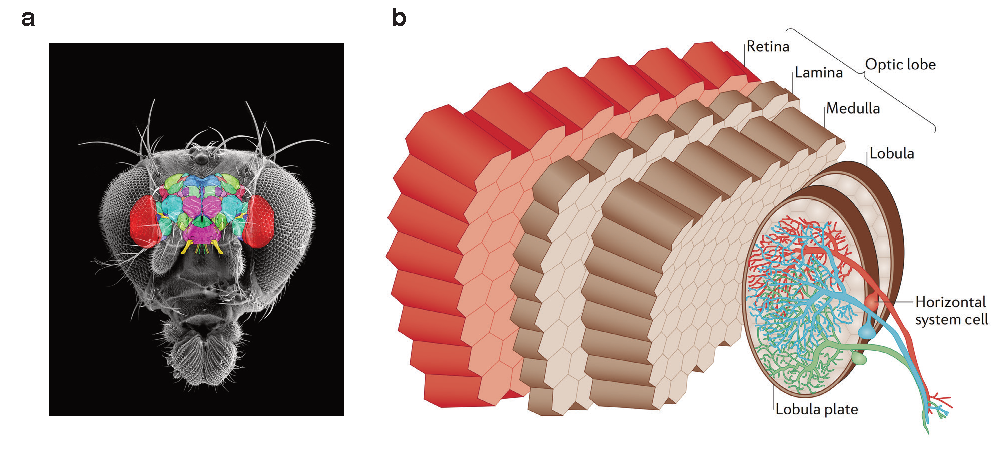
\includegraphics[width=1.0\textwidth]{graphics/figure_lobe}
    \caption[Anatomy of the fly visual system]
    {Anatomy of the fruit fly nervous system. \textbf{a} Schematic of the fly brain overlaid onto a picture of the \textit{Drosophila} head. Illustration from \citet{Ito:2014aa}. \textbf{b} Gross anatomy of the fly optic lobe, divided into retina, lamina, medulla, and the lobula complex consisting of lobula and lobula plate. Neuron schematics depict three tangential cells of the horizontal system (HS). Illustration from \citet{Borst:2014kl}.}
    \label{fig:anatomy}
\end{figure}

In concert, the techniques of circuit neuroscience have painted a made great strides toward a detailed picture of how motion is computed in the visual system of flies. At the level of gross anatomy the fruit fly brain consists of two parts, a thoracic ganglion and a central brain located in the head (Figure \ref{fig:anatomy}a). Estimates put the overall number of neurons on the order of $10^6$ cells\footnote{\citet{Benzer:1967aa} remarks that scaled logarithmically, this puts the fly nervous system halfway between a single neuron and the human brain.} \citep{Morante:2004aa}. A significant portion of these units, possibly more than half, is devoted to the processing of visual information. This occurs primarily in the optic lobes located immediately behind the prominent compound eyes (Figure \ref{fig:anatomy}b). The subunits of this ganglion---lamina, medulla, and a lobula complex consisting of lobula plate and lobula---exhibit an interesting combination of stereotypy and cellular diversity, with clearly repetitive columns dominating high-level structure but the number of distinct neural types exceeding a hundred \citep{Fischbach:1989uw}.

The following sections introduce the neural structure of the \textit{Drosophila} optic lobe, seen through the lens of function and specifically motion vision. Where suitable, I reference the rich history of inquiry into motion detection in larger flies given that many mechanisms are thought to be preserved among dipteran species.

%%%

\subsection{Retina}
All sensory systems start at transduction, the process of transforming physical signals of interest into the activity of sensory neurons. In fruit fly vision, this is achieved by photoreceptors in the retina that convert impinging light into electrical signals. This yields time- and space-resolved signals from which visual cues like color, motion, or object position can be computed downstream. Critically, incoming optical signals are projected into a sensor-centric, two-dimensional coordinate system where each "pixel" corresponds to some location in retinotopic space.

The compound eye of the fruit fly comprises $\approx 800$ hexagonally laid-out ommatidia or facets whose average axial separation is slightly below $\SI{5}{\degree}$ \citep[for a detailed map of the somewhat inhomogeneous fruit fly eye, as compiled by Erich Buchner, see][]{Heisenberg:1984aa}. Each ommatidium has an acceptance angle of half-width $\approx \SI{5}{\degree}$ \citep{Goetz:1965aa}. Resolution and visual acuity of \textit{Drosophila} are thus comparatively low \citep{Land:1997aa}. In contrast to "simple" single-lens configurations like the mammalian eye, each facet has its own optical system that focuses incoming light onto a set of eight photoreceptors per ommatidium. The sensory neurons separate into six outer (R1 through R6) and two inner units (R7 and R8). These receptors are highly sensitive as well as incredibly fast due to an amplifying and adaptive transduction cascade that scales from single photon incidences to day-light conditions separated by many orders of magnitude \citep{Hardie:2001aa,Hardie:2015aa}.

To maximize interaction surface, the inside of the photoreceptor is lined with $\approx\num{30000}$ microvilli, each containing the machinery for transduction. Together, they form the wave-guiding rhabdomere. The transduction cascade is initiated when photons are absorbed by rhodopsin which induces the metarhodopsin state via photoisomerization. Interestingly, while the vertebrate cascade requires time-intensive reconstitution of rhodopsin through enzymatic pathways, re-isomerization in flies is simply achieved by exposure to longer-wavelength light. Shielding pigments in the \textit{Drosophila} eye are transparent to these wavelengths, giving them their characteristic red color. Scattering light can therefore continuously and efficiently reset the cascade. Following isomerization, rhodopsin induces the dissolution of the G-protein Gq whose $\alpha$-subunit in turn binds to a phospholipase C (PLC) isoform encoded by \textit{norpA}. As expected, flies with mutations in this locus are blind \citep{Bloomquist:1988aa}. Via some still partially unmapped mechanism, PLC activation gates transient receptor potential channels, the calcium-conducive TRP and TRPL, which finally depolarize the cell. There is intriguing evidence that the PLC-controlled opening of TRP channels involves a mechanical step, contraction of the cell membrane \citep{Hardie:2012aa}. In \textit{Drosophila} this cascade can operate incredibly quickly: single-photon responses are \SIrange{10}{100}{\times} faster than those in mammalian rod photoreceptors, explaining flicker fusion frequencies in excess of \SI{200}{\hertz} \citep{Heisenberg:1984aa,Hardie:2015aa}.

Wavelength sensitivity is largely determined by the absorption profile of the rhodopsin. R1-6 express the \textit{ninaE}-encoded wide-spectrum opsin \textit{Rh1} with sensitivity that peaks twice, once in the ultraviolet and once in the green range. They provide high-resolution input to achromatic visual behaviors like motion vision. Mutations that affect R1-6 or \textit{rh1} as well as genetic silencing of R1-6 through specific expression of UAS-Shibire\textsuperscript{ts1} drastically impair both optomotor and fixation response \citep{Heisenberg:1977aa,OTousa:1985aa,Rister:2007fn}. R7 and R8, on the other hand, contain stochastic combinations of more sharply tuned single-peak rhodopsins \citep{Franceschini:1981aa} and mediate spectral behaviors like color discrimination at low spatial resolution \citep{Schnaitmann:2013aa}. Their inactivation does not substantially affect motion-guided behavior \citep{Yamaguchi:2008aa}, but some have argued that R7 and R8 activity shapes R1-6 responses through gap junctions \citep{Wardill:2012aa}.

An interesting complication arises from the fact that the outer photoreceptors have slightly offset optical axes due to the geometry of the ommatidium that houses them; R1 through R6 thus point in slightly different directions in visual space. If the mapping from ommatidia to downstream cartridges, each processing signals from a point in the visual field, was one-to-one, summation of the photoreceptors would significanctly lower spatial acuity. Instead, \textit{Drosophila} makes use of neural superposition. Photoreceptors with parallel optical axes from neighboring ommatidia are routed into the same cartridge downstream, forming a neuro-cartridge whose inputs are properly aligned \citep{Trujillo:1966aa,Braitenberg:1967aa}. This sophisticated wiring scheme preserves acuity while maximizing sensitivity through pooling of multiple receptors and outperforms the apposition or optical superposition eyes of other arthropods \citep{Kirschfeld:1967aa}.

\subsection{Lamina}

\subsubsection{Structure}
Axons of retina photoreceptors project into the first neuropil of the optic lobe, the lamina. It consists of eight strictly repeated cell types that are arranged in retinotopic columns corresponding to the neuro-cartridges outlined above. That is, visual information from adjacent points in visual space is processed in anatomically adjacent modules of the lamina \citep{Fischbach:1989uw}. Lamina monopolar cells L1-5 are the most prominent instances of these periodic neurons, providing feedforward signals to various layers of the subsequent neuropil, the medulla. Centrifugal neurons C2 and C3 as well as T1, on the other hand, receive dendritic input in the medulla and send what is generally presumed to be feedback connections into the lamina. In addition to this set, there are four infra-periodic cell types whose arbors span multiple columns: lamina wide-field neurons Lawf1 and Lawf2 which receive input from the medulla, the lamina-tangential neuron Lat which connects central brain and lamina, and the lamina-intrinsic neuron Lai.

Electron microscopy studies have shed significant light on lamina connectivity \citep{Meinertzhagen:1991aa,RiveraAlba:2011dd}. Only L1-3 receive direct input from photoreceptors R1-6 although there is evidence that L4 is post-synaptic to at least R6. L1 and L2 are known to be electrically coupled \citep{Joesch:2010fw}, and L2 forms a reciprocal sub-network with L4 cells in its own as well as neighboring columns. Far from being neatly segregated, column-intrinsic lamina networks therefore exhibit substantial complexity. While C2 and C3 synapse onto multiple lamina targets, nothing is known about within-lamina connectivity of T1. The connectivity of multicolumnar feedback neurons is somewhat diffuse, with Lawf1 and Lawf2 for instance connecting to multiple cells. While the neurotransmitter identity of most lamina cells remains mysterious, \citet{Takemura:2011iy} could establish L1 as glutamatergic and both L2 and L4 as cholinergic using transcript profiling in single cells.

\subsubsection{Function}
Monopolar cells L1-3 express an \textit{hcla}-encoded, \textit{ort}-dependent chloride channel that is gated by photoreceptor-released histamine \citep{Hardie:1989aa,Gengs:2002aa}. Physiological response properties of lamina monopolar cells were first described in larger fly species where comparatively large cell bodies permit electrophysiological recordings with sharp electrodes \citep{Laughlin:1978aa,Laughlin:1981wn,Laughlin:1989aa}. Photoreceptors depolarize in response to light. Lamina monopolar cells, on the other hand, hyperpolarize transiently in response to step-like illumination, followed by weaker sustained polarization. When the stimulus is switched off, rebound depolarization occurs. All signalling occurs via graded potentials. Lamina processing is therefore well approximated by inverting and high-pass filtering the photoreceptor voltage response which could be expected from the conductance profile of the involved channels. Critically, lamina cells are not selective for direction.

More recently, genetically encoded calcium indicators have made it possible to directly record response properties of identified lamina cells in the fruit fly. L1 and L2 respond identically and in line with blowfly findings to luminance changes \citep{Reiff:2010eo,Clark:2011gw} while L4 and particularly L3 exhibit less transient response dynamics \citep{Silies:2013jp,Meier:2014fr}. Moreover, L2 receptive fields display a noticeable inhibitory surround that contributes to their size selectivity and differentially shapes temporal response characteristics \citep{Freifeld:2013gu}. In contrast, L4 responses appear to pool from large parts of the visual field, suggesting an intriguing role for electric coupling within this lamina network \citep{Meier:2014fr}. Patch-clamp recordings from lamina wide-field neurons revealed sensitivity to slow oscillations in luminance, hinting that these neurons provide feedback about lighting conditions to lamina circuits \citep{Tuthill:2014gc}.

The combination of direct lines L1-3 and indirect relays L4-5 provides heavily multiplexed visual information to downstream medulla circuits. This suggests a form of division of labor when it comes to computations and behaviors mediated by their input. Genetic silencing via GAL4-UAS has allowed multiple studies to examine such functional differences, particularly between the large monopolar cells L1 and L2. \citet{Rister:2007fn} could show in behavioral tasks that blocking both cells in conjunction renders flies optomotor-blind, emphasizing the critical contribution of L1 and L2 to the detection of motion. Moreover, their experiments tentatively suggested that the L1 and L2 pathways mediate the extraction of particular directions of retinal optic flow (back-to-front versus front-to-back, respectively). Other studies implicated L2 specifically in looming detection or the regulation of translational velocity \citep{deVries:2012aa,Katsov:2008iy}. A critical insight came from the use of contrast-specific stimuli. When stimulating with bright (ON) or dark (OFF) traveling edges, electrophysiological recordings in motion-sensitive tangential cells of the lobula plate revealed a strong divergence between L1 and L2 block phenotypes \citep{Joesch:2010fw}. When L1 was silenced, ON responses were strongly reduced while leaving the other polarity unaffected. Conversely, when L2 was silenced, only OFF responses were abolished. This indicated that similarly to the vertebrate retina, the fly visual system computes motion separately for stimuli defined by positive and negative contrast. L1 then provides the input to an ON pathway and L2 to an OFF pathway. Behavioral experiments later found comparable phenotypes in walking and flying \textit{Drosophila} \citep{Clark:2011gw,Tuthill:2013jk}. Moreover, \citet{Reiff:2010eo} found evidence of appropriately signed half-wave rectification in flash responses of L2 axon terminals in the medulla \citep[which may differ in dynamic stimulus regimes, see][]{Clark:2011gw,Strother:2014aa}.

There is still considerable uncertainty about the particular functional roles that lamina pathways other than L1 and L2 play. L3 has been associated with chromatic processing \citep{Gao:2008ik}, but \citet{Silies:2013jp} propose that the monopolar cell is also involved in OFF motion processing. Recording from tangential cells in the lobula plate, \citet{Meier:2014fr} observed abolished OFF motion responses after silencing L4 which again points towards interesting interactions within the local sub-network of L2 and L4. Finally, a large-scale behavioral screen in which all twelve lamina cells were silenced individually could not reveal clear phenotypes for lamina units outside of L1 and L2 \citep{Tuthill:2013jk,Tuthill:2014gc}.

\subsection{Medulla}

\subsubsection{Structure}
The major target of lamina monopolar cell axons is the medulla, a secondary structure of the optic lobe. It is characteristically stratified and consists of ten layers (M1 through M10), clearly separable by determining projection patterns and arborization \citep{Fischbach:1989uw}. Processing in the medulla remains retinotopic but crosses along the anterio-posterior axis within the neuropil-separating chiasm. Here, representations fan out drastically. More than 60 columnar cell types can be distinguished based on morphology and ramifications, presumably providing a large number of specialized visual channels to downstream circuits. Medulla neurons send parallel projections into both neuropils of the lobula complex and fall into at least three categories:

\begin{itemize}
    \item Medulla-intrinsic (Mi) cells that connect upper (distal) to lower (proximal) layers of the medulla
    \item Trans-medulla (Tm) cells whose projections go beyond the medulla, predominantly into the lobula
    \item Trans-medulla Y cells (TmY) whose projections bifurcate, reaching both lobula and lobula plate
\end{itemize}

In addition, one can identify the so-called "bushy" T cells (T2-5) that appear multiple times per column. While T2-4 receive input within the confines of the medulla, T5 connects lobula and lobula plate. T4 and T5 share a particular projection pattern with individual units targeting specific strata of the four-layered lobula plate. For this reason as well as due to functional considerations, I discuss T5 in the section at hand\footnote{Indeed, some studies hold that the lobula and particularly the lobula layers in which T5 cells ramify originated from proximal strata of the medulla that were displaced in the course of evolution \citep{Douglass:1996aa,Shinomiya:2015aa}.}. T4 and T5 can be classified into four sub-types, T4a-d and T5a-d, which project into distinct downstream layers. The two types are therefore classified as hypercolumnar \citep{Bausenwein:1992vx}. Crucially, they are the only cells that project retinotopically from medulla and lobula into the lobula plate where wide-field motion-sensitive tangential cells are located \citep{Fischbach:1989uw,Douglass:1996aa}.

Through electron microscopy studies, projections of lamina monopolar cells in the upper layers of the medulla have been mapped in great detail \citep{Takemura:2008ee}. L1 and L5 arborize in layers M1 and M5, L2 in layer M2, L3 in layer M3, and L4 in layers M2 and M4. Interestingly, R7 and R8 extend axons that bypass the lamina and directly target distal layers of the medulla. Such patterns have guided hypotheses about connectivity between lamina and medulla cells. The arborization pattern of trans-medulla cell Tm2, for instance, suggested that it receives input from L2. This could later be confirmed by further reconstruction efforts \citep{Takemura:2011iy}.

\citet{Bausenwein:1992vx} analyzed Golgi stainings of the medulla cells and proposed at least two major pathways connecting lamina to lobula plate via medulla and lobula. One consists of the sequence L1, Mi1, and T4 and the other involves L2, Tm1, and T5. Recent connectomic efforts within the medulla have started to complete this picture. \citet{Takemura:2013ea} could confirm the L1-Mi1-T4 chain and put forward Tm3 as another critical input to T4. Similarly, \citet{Takemura:2011iy} implicated Tm2 in the pathway downstream of L2, with further projections arising from connections within the L2-L4-Tm2 circuit. Subsequent reconstructions traced connections from Tm1 and Tm2 onto T5 and found that medulla neurons Tm4 and Tm9 also synapse onto T5 dendrites in the lobula \citep{Shinomiya:2014dx}. Interestingly, Tm9 receives its dominant lamina input from L3. In light of the functional division between ON and OFF pathways shown through silencing experiments involving L1 and L2, these medulla circuits emerged as likely candidates for the neural implementation of motion detection. Critically, however, any such anatomical model requires confirmation through functional studies.

\subsubsection{Function}
Neural processes in the medulla are numerous, densely packed, and heavily intertwined. In combination with the small size of associated cell bodies, this has greatly hindered characterization of their visual response properties and turned the medulla into the "terra incognita" of the fly optic lobe. Even for larger flies like \textit{C. vicina} only sparse electrophysiological data exist, collected predominantly from unidentified units \citep{Mimura:1972aa,DeVoe:1980aa,Douglass:1995aa,Douglass:1996aa}. An interesting approach for identifying motion-relevant medulla pathways based on 2-deoxyglucose activity labeling under visual stimulation was pursued by \citet{Bausenwein:1992aa}. They used a comprehensive set of patterns that included rotating and expanding square-wave gratings as well as isolated traveling stripes. Post-hoc analysis of staining distributions within the fruit fly medulla corroborated the two motion-related pathways anatomy had suggested, again indicating that T4 and T5 may be critical motion-relevant projections to the lobula plate.

Optical interrogation methods like GAL4-targeted two-photon calcium imaging have now made headway toward understanding signal processing that occurs in the medulla. \citet{Meier:2014fr}, for instance, used this technique to record visual response properties of Tm2 terminals in the first layer of the lobula. Tm2 cells respond preferentially to OFF edges and are themselves not selective for direction. Taking a different approach, \citet{Behnia:2014jh} characterized a subset of candidate motion circuit cells using GFP-guided patch clamp. Their work demonstrated that presumed ON pathway cells Mi1 and Tm3 depolarize in response to brightening stimuli; OFF pathway cells Tm1 and Tm2, on the other hand, depolarize in response to darkening stimuli. None of the cells were themselves direction-selective. Quantification of their output kinetics revealed exceedingly small differences between time constants of each pair, which were proposed to underlie motion selectivity following non-linear combination downstream. In a first approximation, this agreed with the division into two pathways originating from L1 and L2, respectively, that genetic silencing approaches and anatomy had supported \citep{Joesch:2010fw,Takemura:2013ea}.

Electrophysiological evidence from the blowfly indicated that T4 cells are not selective for direction, but these studies were unable to reliably establish cell identity and suffered from low yield \citep{Douglass:1996aa}. Two key findings in \textit{Drosophila}, however, made T4 and T5 promising candidates for the task of relaying motion information to the lobula plate. First, when they were genetically silenced using either UAS-Kir2.1 or UAS-Shibire\textsuperscript{ts1}, motion responses in lobula plate tangential cells downstream of the medulla were fully abolished \citep{Schnell:2012iz}. Second, the same block flies could be shown to be completely optomotor-blind when tested on a treadmill set-up \citep{Bahl:2013ha}. Yet, the exact role of T4 and T5 in computing motion as well as potential functional differences still awaited clarification.

\subsection{Lobula complex}

\subsubsection{Structure}
Two separate neuropils, lobula and lobula plate, together form the lobula complex. As mentioned above, medulla projections bifurcate and target the two downstream structures in parallel. Additionally, lobula processes connect to the lobula plate, most saliently among them the four sub-classes of T5 \citep{Fischbach:1989uw}. Both structures are stratified; based on arborization patterns and morphology, the lobula can be subdivided into at least six layers and the lobula plate into four.

The lobula complex is the major source of projections from the optic lobe to other areas of the fly brain. Comparatively little is known about lobula projection neurons, both functionally and structurally, but anatomical characterizations have revealed LC neurons as a numerous and heavily subdivided class that collectively spans the retinotopic representation of visual space in the lobula \citet{Otsuna:2006aa}.

In contrast and due to its role in motion processing, the lobula plate particularly of larger dipteran species has received a great deal of anatomical and functional attention over the past decades \citep[for thorough reviews, see][]{Borst:2002iw,Borst:2010fk}. Large tangential cells represent the most striking group of neurons in the lobula plate. Based on anatomy and response characteristics, over 60 so-called lobula plate tangential cells (LPTCs) could be described in \textit{C.\ vicina}. The tremendous dendritic trees of individual LPTCs sample input from hundreds of columns and thus large portions of visual space. Individual processes can reach diameters close to \SI{10}{\micro\meter}. The ramifications of LPTCs are often highly specific. Cells of the horizontal system (HS), for instance, receive input from frontal layers of the lobula plate while vertical system (VS) cells arborize primarily in the posterior part. The mapping of the \textit{Drosophila} lobula plate is less complete. However, several studies have been able to identify corresponding LPTCs that closely match their counterparts in larger flies \citep{Fischbach:1989uw,Scott:2002aa,Joesch:2008fo,Schnell:2010ik}.

From the lobula complex, projections take three major routes. Lobula neurons primarily target optic glomeruli in the lateral protocerebrum \citep{Mu:2012aa}. Axons of LPTCs either go to motor areas of the thoracic ganglion via descending neurons or directly to neck motor neurons that govern head movement \citep{Strausfeld:1985aa,Borst:2014kl}.

\subsubsection{Function}
Due to their size and accessibility, LPTCs have been prime targets for electrophysiological studies in "big" flies \citep{Hausen:1976aa,Hausen:1982aa,Hausen:1982bb,Hengstenberg:1982aa,Borst:2010fk} and even \textit{Drosophila} \citep{Joesch:2008fo,Schnell:2010ik}. They respond to motion in a direction-selectively opponent fashion and have receptive fields that extend over substantial parts of the visual field. HS cells, for example, depolarize when stimulated with front-to-back motion and hyperpolarize in response to the opposite direction. For VS cells, the preferred direction is downward. In the fruit fly, at least three HS cells (HSN, HSE, and HSS) and six VS cells (VS1-6) have been identified \citep{Joesch:2008fo,Schnell:2010ik}. A significant fraction of LPTCs signals via graded potentials; others, like H1 in \textit{Calliphora}, spike. Interestingly, the cells recapitulate many of the properties of the optomotor reflex. Under sinusoidal stimulation, the response magnitude has an optimum and depends on wavelength and contrast of the pattern. Indeed, similarly to the optomotor response, LPTCs are tuned to the contrast frequency $\frac{v}{\lambda}$ of a drifting grating. Sensitivity peaks in the range of \SIrange{0.5}{1}{\hertz}.

Multiple lines of evidence have linked these cells to visually guided locomotion. When motion receptive fields of LPTCs are measured at high spatial resolution, they resemble filters that are matched to the optic flow generated by particular maneuvers. VS cells in \textit{Calliphora}, for instance, are tuned such that they are maximally activated by input that would result from rotation around specific horizontal body axes \citep{Krapp:1996}. Similar logic holds for other LPTCs like HS and corresponding units in the fruit fly \citep{Krapp:1998aa,Schnell:2010ik}. This suggests that tangential cells act as ego-motion sensors, allowing the fly to monitor and correct its head orientation and trajectory based on visual input. Intrinsic connections as well as contralateral projections appear to play critical roles in tuning this optic flow-processing network \citep{Borst:2011kk,Weber:2012dr}. For instance, there is evidence that electric coupling within sub-networks like VS further refines flow field selectivity \citep{Haag:2004ho}. Finally, micro-surgical ablations of LPTCs as well as mutations that affect the lobula plate produce specific impairments of associated head or body movements \citep{Heisenberg:1978aa,Geiger:1981aa,Hausen:1983js}.

The layer-specificity of LPTC dendrites has critical functional relevance. Using deoxyglucose-based activity mapping while stimulating fruit flies with moving gratings, \citet{Buchner:1984aa} could show that the four layers of the lobula plate respond to motion along four cardinal directions in visual space: front-to-back (layer 1), back-to-front (layer 2), upward (layer 3), and downward (layer 4). This is compatible with the observation that LPTCs ramify in layers matching their preferred direction \citep{Heisenberg:1978aa,Schnell:2010ik}. The identity of the relevant projection cells as well as the locus of motion detection, however, have proven elusive.

Little is known about visual response properties of lobula projection neurons. Nonetheless, studies on various fly species have suggested a wide range of stimulus selectivity in the lobula complex, including cells that respond preferentially to looming patterns \citep{deVries:2012aa}, figure-ground motion \citep{Egelhaaf:1985aa}, or movement of small objects \citep{Barnett:2007fp}.

\section{Algorithmic models of motion detection}
What is required before one can reasonably claim to understand any given system? A popular answer---particularly in the tradition of cybernetics---comes in the form of modeling, the process of building artificial mechanisms that emulate the computations and behaviors accomplished by real brains. If we can replicate what any given neural circuit is doing, and ideally do so quantitatively, substantial progress toward understanding has been made. Models then allow us to isolate minimally required elements, explain existing variance, and predict new results, thus driving subsequent experimental work. They come in many forms, ranging from the simplified and abstract (such as regression or filters) to the complex and concrete (such as biophysical cell models or recurrent neural networks).

\citet{Yamins:2016hg} identify three qualities that models of sensory systems should possess:
\begin{itemize}
    \item Stimulus-computability (the ability to accept arbitrary stimuli within the relevant domain)
    \item Mappability (an internal structure that can be compared to neural circuitry)
    \item Predictivity (the ability to compute output for individual stimuli, particularly ones not seen during model fitting)
\end{itemize}
While formulated in the context of visual cortical processing, I argue that these demands apply to sensory models in general. Of course, an additional constraint comes from simplicity. If possible, models ought to be as intricate as necessary but no more. With increasing numbers of parameters and general unwieldiness, models run the risk of over-fitting particular data sets and lose their ability to pinpoint critical computational principles \citep[for an example of a large-scale model of presumably limited explanatory value, see][]{Markram:2015aa}. 

Motion vision offers a noteworthy example for the productive interplay between experiment and modeling. Early attempts at explaining the psychophysics of motion perception in a connectivist model can be traced back to \citet{Exner:1894aa}. However, his circuit scheme was quantitative only in the vaguest sense. \citet{Hassenstein:1956fa} then made the crucial step toward an algorithmic description of motion processing, one that related motion stimulus to graded behavioral responses using the rigorous tools of signal processing theory. Decades of subsequent research have shown that this detector beautifully fulfills the criteria outlined above. In the following section, I review major models for motion detection in the specific context of fly vision.

\subsection{Fundamental requirements}

Motion of objects has a simple physical definition, displacement over time. Velocity is then given by the elementary difference
\begin{equation}
    v = \frac{\mathop{dx}}{\mathop{dt}}
\end{equation}
where $x$ denotes position and $t$ time. Direction is easily extracted by identifying the sign of $v$. If a motion algorithm had access to high-level features like object position, then motion estimation would be a simple task. However, there is strong evidence that animals from fly to primate extract directional signals directly from simple luminance signals \citep{Borst:2011bq,Adelson:1985tx}.

% An interesting static approach comes from Fourier analysis of motion \citep{vanSanten:1985ug}. For any rigidly translating one-dimensional image, the amplitude spectrum of the space-time representation consists of a single line through the origin. Its slope is fully determined by the velocity of the translation. The logic naturally extends to two-dimensional input. A system that has full access to the spatio-temporal history of the visual stimulus could feasibly retrieve motion by measuring the parameters of this line. Such a computation has indeed been suggested for computer vision applications \citep{Heeger:1987ti}. However, it seems obviously implausible for simple nervous systems like that of a fly which transform continuous input and do so instantaneously.

The geometry of motion dictates some basic requirements that any such detector must satisfy \citep{Borst:1989vp}:

\begin{enumerate}
    \item Signals have to be sampled at a minimum of two spatial locations. Any input from one location (which \citet{Reichardt:1987uo} calls a 1-input graph), is inherently ambiguous with regard to direction.
    \item The two signals have to be processed asymmetrically. If the detector is mirror-symmetrical, flipping the stimulus along the axis of motion has no effect on the output even though the direction reverses.
    \item Input signals have to be combined in a non-linear fashion. Linear motion filters can be constructed and signal direction under certain constraints \citep[see for instance][]{Watson:1985tl}. In general, however, they fail to model empirical direction-selectivity as their time-averaged output is equivalent to the time-averaged input signals, thereby discarding critical information about stimulus sequence.
\end{enumerate}

In the next part, I discuss the two major classes of motion algorithms that fit the outlined criteria.

\subsection{Gradient detectors}
If one has access to a local gradient of the luminance pattern $I(x,t)$ across space $x$ and time $t$, then stimulus velocity is readily obtained from the relation
\begin{equation}
    \frac{\mathop{\partial I}}{\mathop{\partial t}} = \frac{\mathop{\partial I}}{\mathop{\partial x}} v
\end{equation}
through division of the temporal gradient by the spatial gradient. The scheme was first described in the context of computer vision \citep{Limb:1975aa,Fennema:1979aa} and has several appealing properties. For instance, its output is proportional to local and instantaneous velocity and does not depend on geometrical properties of the stimulus like pattern wavelength or contrast. Moreover, for a fixed-velocity stimulus the estimate is constant in time. Several studies have successfully applied this detector model to the study of biological motion vision \citep{Hildreth:1987jt,Johnston:1995aa,Borst:2007gz}.

It is of course unlikely that biological realizations of the gradient detector compute fully localized derivatives. Neurally plausible models commonly estimate the spatial derivative as a finite difference between two luminance-sensitive receptors sampling spatially displaced image locations. They then approximate temporal differentiation through mean adaptation as realized by, say, a basic high-pass filter \citep{Srinivasasn:1990aa,Borst:2011bq}.

To operate effectively, the detector clearly requires robust approximations of the luminance gradient. A divisive non-linearity confers several advantages, such as invariance to stimulus contrast, but fails under challenging stimulus conditions. For instance, if pattern contrast is low, spatial derivatives may approach zero and cause the velocity estimate to either amplify random fluctuations of the temporal gradient or become undefined. For vision, the problem is exacerbated by the Poisson statistics of photon incidence. Such "shot noise" makes photoreceptor output unreliable under low-light conditions \citep{Laughlin:1996aa}. Simulations indicate that for input conditions dominated by noise, the information rate of gradient detectors drops dramatically \citep{Borst:2007gz}.

Some formulations circumvent the issue through non-linearities that are less dependent on stable estimates of the gradient, like the logical veto gate put forward by \citet{Marr:1981aa}. \citet{Potters:1994aa} suggested that motion vision should only be mediated by gradient detectors in the regime of large signal-to-noise ratios. If stimuli are noisy, more robust algorithms like the correlation detector described below ought to be preferred. Counter to this dual-mechanism postulate, \citet{Haag:2004bj} could show that blowfly motion vision exhibits the hallmarks of correlation-based schemes across a wide range of pattern luminances. The proposed trade-off between mechanisms was not observed.

\subsection{Correlation detectors}

Correlation detectors represent the predominant class of motion extraction models used in sensory neuroscience. They have successfully been employed to explain properties of motion vision across a wide spectrum ranging from psychophysics and animal behavior down to physiological responses of direction-selective cells.

Fundamentally, the algorithm is based on the asymmetrically delayed comparison of two spatially separated visual inputs. This lines up well with physical intuitions about motion. When an object moves from one location to the next, we observe a visual match across time and space. A bright dot moving from left to right, for instance, produces first a positive deflection in the output of the leftmost photoreceptor and then, after a time determined by the object's velocity, a positive deflection in the adjacent rightward location. In a sense, motion detection then reduces to the task of determining the temporal sequence of these two visual events. The logic conveniently extends to continuous luminance signals. By isolating slanted spatiotemporal correlations, one can compute the direction and magnitude of motion from locally sampled brightness input. The operation then closely resembles cross-correlation of two spatially separated inputs \citep{Reichardt:1987uo}.

\subsubsection{Reichardt detector}

The first quantitative description of a correlation-type motion detector was derived from optomotor behavior in \textit{Chlorophanus viridis} walking on a Y-maze \citep{Hassenstein:1951aa}. Their textured rotating drum was only observed through a pair of separated slits, so the stimulus consisted of two spatially and temporally isolated brightness changes resembling apparent motion \citep{Wertheimer:1912aa}. Hassenstein showed that the beetle would robustly turn with pattern motion if the events had the same contrast polarity. That is, combinations of either two bright (ON) or two dark (OFF) events elicited syndirectional turning. However, for mixed-polarity sequences (ON-OFF or OFF-ON) turning was inverted. This response is closely related to the psychophysical phenomenon of reverse-phi \citep{Anstis:1970tv,Anstis:1975tu}. When \citet{Hassenstein:1956fa} varied spatial and temporal separation of the flashes, they found clear optima. Critically, the ideal spatial separation was approximately equivalent to beetle's inter-ommatidial distance.

A critical insight for model building came from analogy to the rules of sign-correct multiplication. Equally signed products are positive, mixed products negative. This led to the development of what is interchangeably called Hassenstein-Reichardt correlator, Reichardt detector, or elementary motion detector \citep{Reichardt:1961aa}. It computes local motion and can operate directly on continuous luminance signals, thus processing arbitrary visual inputs.

\begin{figure}
    \centering
    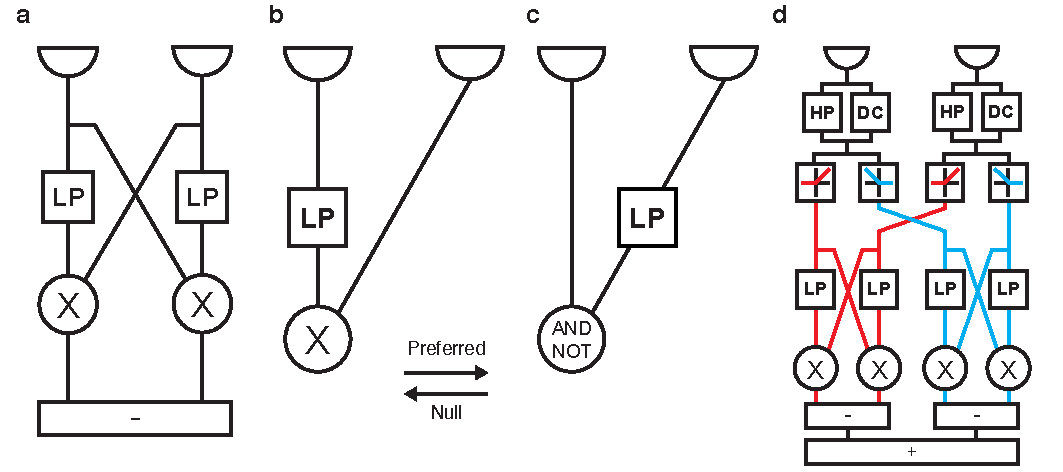
\includegraphics[width=1\textwidth]{graphics/figure_models1}
    \caption[Correlation-type models for motion detection]
    {Architecture of basic and elaborated correlation detectors. \textbf{a} Fully opponent Reichardt detector based on multiplication of spatially separated, asymmetrically filtered inputs. It responds positively to preferred rightward and negatively to null leftward motion. \textbf{b} Reichardt-type half-detector using facilitation of preferred motion. \textbf{c} Barlow-Levick half-detector. Note that here, the non-linearity is a veto gate and the delay has switched sides to maintain preferred direction. \textbf{d} Elaborated Reichardt detector derived from findings on polarity specialization in the \textit{Drosophila} visual system \citep{Eichner:2011ic}.}
    \label{fig:detector1}
\end{figure}

%%%

In its basic form, the detector consists of two mirror-symmetrical subunits (Figure \ref{fig:detector1}a). Each receives visual input from two distinct points in visual space separated by the sampling distance $\Delta\phi$, one of which is then delayed with respect to the other. This processing step can take many forms, including a true delay that leaves the signal otherwise unchanged, but is often implemented as a first- or second-order linear temporal filter. Such low-pass filters incur a phase shift that effectively delays arbitrary time-varying signals. Subsequently, the two signals are multiplied.

This combination of filtering and multiplication implements the delay-and-compare algorithm described above: if $\Delta\phi$ and the time constant of the delay filter are matched to the direction and velocity of the traveling object, two signal deflections will coincide at the multiplier and give rise to a large signal. This happens only when the object first passes the delayed line, therefore moving along the preferred direction of the subunit. Conversely, if the object moves in the opposite (or null) direction, excitations are mistimed and produce small or no output. Finally, the output signals of the two oppositely tuned subunits are subtracted. This results in a fully opponent direction-selective detector that responds positively for its preferred and negatively for its null direction. Additionally, the subtraction stage suppresses signals produced by motion-unrelated visual cues like static illumination or full-field flicker. Under the assumption that each ommatidium provides one such input signal, the algorithm parsimoniously explains the aforementioned findings on optomotor responses in the beetle. In particular, it predicts the inversion that occurs when negative and positive contrast are combined in appropriately spaced spatial and temporal succession. Its architecture also adheres to the three criteria listed in the previous section, with multiplication supplying the non-linearity \citep{Borst:1989vp}.

Any elementary motion detector is only sensitive to motion within the small part of the visual field defined by nearest-neighbor interactions of inputs. To generate the behavioral optomotor response, \citet{Hassenstein:1956fa} proposed that a large array of detectors is spatially integrated. When stimulated with periodic sine gratings traveling at a fixed velocity, individual detectors produce sinusoidally modulated output. Direction is encoded in the offset or temporal mean of the response. After summation, responses still show some initial oscillations. However, the steady-state response does not vary with time. The length of this modulated period is determined by the filter time constants of the input lines \citep{Egelhaaf:1989wf,Egelhaaf:1989wd}.

Depending on the particular model in question, a different filter configuration may be used; some instantiations have a peripheral high-pass filter in both arms, some only in the non-delayed line, and others only use a single low-pass filter in the delayed line. Qualitatively, response properties of these variations are similar \citep{Borst:2003bz}.

\begin{figure}
    \centering
    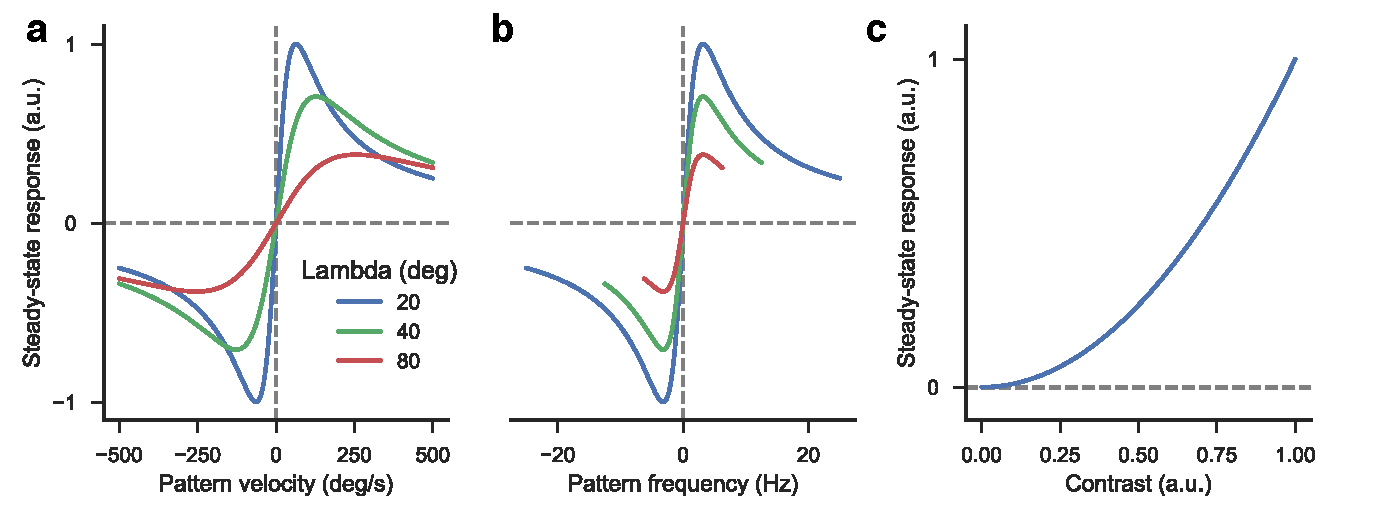
\includegraphics[width=1.03\textwidth]{graphics/figure_rd}
    \caption[Response properties of the Reichardt detector]
    {Response properties of a low-pass-based Reichardt detector array. \textbf{a} Velocity tuning for simple sinusoidal gratings. The value of the response optimum depends on pattern wavelength $\lambda$. \textbf{b} Data from \textbf{a} replotted on a frequency scale. Peaks now align, indicating that the detector is tuned to contrast frequency. \textbf{c} Responses also depend quadratically on contrast. The simulated detector array consisted of 50 units with \SI{50}{\milli\second} time constant and a receptor distance of \SI{5}{\degree}.}
    \label{fig:tuning}
\end{figure}

For specific forms of the Reichardt detector, the steady-state frequency optimum can be calculated analytically. Consider a simple model that has a first-order linear low-pass filter with time constant $\tau$ in the delayed arm and passes the signal unfiltered in the direct line. The time- and space-averaged steady-state response of the array is then given by
\begin{equation}
    R = {\Delta I}^2 \sin(2 \pi \frac{\Delta\phi}{\lambda}) \frac{\tau \omega}{1 + \tau^2 \omega^2}
\end{equation}
where $\mathop{\Delta I}$ denotes grating contrast, $\lambda$ the spatial wavelength of the pattern, and $\omega$ the circular contrast frequency $2 \pi f$ \citep{Borst:2003bz}.

From this, we can see that Reichardt detector arrays neatly recapitulate the fundamental tuning properties of the grating-induced \textit{Drosophila} optomotor response \citep{Gotz:1964bj} as well as functional properties of tangential cells \citep{Joesch:2008fo}:

\begin{enumerate}
    \item The sign of the response depends on the direction of the moving pattern (Figure \ref{fig:tuning}a).
    \item The velocity tuning hinges critically on the spatial wavelength of the pattern and the detector is tuned to temporal frequency $\frac{v}{\lambda}$  (Figure \ref{fig:tuning}b).
    \item The frequency tuning has an optimum (Figure \ref{fig:tuning}b).
    \item When the stimulus is under-sampled, responses invert (as indicated by the $\Delta\phi$-dependent geometric interference term). Setting the sampling base to the inter-ommatidial angle reproduces empirically measured aliasing, supporting the notion that the fly visual system extracts motion from local interactions.
    \item Responses increase quadratically with contrast due to the multiplication stage (Figure \ref{fig:tuning}c).
\end{enumerate}

The close match between a model initially derived from beetle behavior and fly vision data suggests that insects share the basic algorithms underlying motion detection. Correlation-based algorithms appear to be a fundamental solution for the problem of determining spatiotemporal sequence.

In contrast to gradient detection strategies and due to the properties of multiplication, Reichardt correlators are quite robust to spatial gradients that approach zero as well as tolerant of degraded input. The detector's output carries substantial information about motion direction and magnitude even in the presence of strong Poisson noise \citep{Borst:2007gz,Shi:2006du}. This comes at the cost of output that strongly depends on unrelated properties of the pattern and is approximately proportional to velocity only within a limited range. Note, however, that for naturalistic image sets, the output of the Reichardt detector becomes a more reliable read-out of image velocity \citep{Dror:2000cr,Dror:2001wc}.

\subsubsection{Motion energy detectors}
Research on vertebrate vision, including psychophysics in humans, has given rise to the so-called motion energy model of direction-selectivity \citep{Adelson:1985tx,vanSanten:1984wg}. It involves the construction of spatiotemporally oriented filters that operate on luminance signals. When viewed across space and time, moving images exhibit a characteristic tilt whose angle of course depends on direction and velocity. An appropriately tilted filter is then sensitive to image motion that matches its receptive field.

In practice, the approach makes use of an elegant trick to create such filters from non-tilted receptive fields. By combining appropriate one-dimensional filters in space and time, one can create odd and even receptive fields that are linearly separable. Summing them in various combinations yields inseparable, spatiotemporally oriented linear filters. Input sequences are convolved with this set of kernels, squared, and finally summed. The resulting output is selective for direction and explains significant aspects of motion phenomenology.

Interestingly, with mild assumptions about the peripheral filters, the motion energy model can be proven equivalent to the Reichardt detector \citep{vanSanten:1985ug}. The product of differentially delayed signals, as it is calculated in the Hassenstein-Reichardt scheme, reappears in the output of the algorithm proposed by \citet{Adelson:1985tx}. Response properties derived for one therefore generally apply to the other. Both are examples of the more general delay-and-compare strategy. Note, however, that internal structure and intermediate representations differ between the two.

\subsubsection{Barlow-Levick detector}
Following physiological investigations in the rabbit retina, \citet{Barlow:1965aa} proposed a cognate algorithm for motion sensitivity that has been particularly influential in studies on the vertebrate visual system \citep{Borst:2015ko}. Their model is structured like an isolated Reichardt detector subunit (Figure \ref{fig:detector1}b); again, two spatially displaced inputs are compared after one of them is delayed. Instead of multiplication, however, the detector uses a veto gate (Figure \ref{fig:detector1}c). If two signals reach the non-linear stage at the same time, no output is produced. Otherwise, signals pass through. While subunits in a Reichardt detector amplify responses to motion in their preferred direction, Barlow-Levick detectors suppress signals elicited by motion in their null direction. 

Reichardt and Barlow-Levick detectors with identical preferred direction thus differ in the type of non-linearity they employ (amplifying versus inhibitory) as well as the placement of the temporal delay (on the arm passed first by a preferred stimulus versus the second). From a functional perspective, however, their characteristics are strikingly similar.

\subsubsection{Elaborated architectures}
Most models described so far were initially designed as black-box approximations of stimulus-response relationships. Circuit neuroscience is of course interested in the correspondence of algorithm and implementation---which neural elements perform the individual computations that make up the detector model? To advance mappability, we may be interested in neurons that act as direct and delayed line or the biophysics that govern the non-linearity of a Reichardt detector. Of further interest are discrepancies between model layout and implementation. In this section, I give some examples of elaborated detector architectures that provide closer fits with either empirical data or biological substrate.

A typical complication, for instance, concerns peripheral receptor elements. At their most basic, these are samples from a single point in the image plane. This model of their optic properties is of course insufficient. Real ommatidia have acceptance angles that in the case of \textit{D. melanogaster} are well approximated by a Gaussian with a half-width at maximum of $\approx \SI{5}{\degree}$ \citep{Goetz:1965aa}. Real-world simulations thus often apply appropriate spatial blurring at the input stage.

More complex modifications were put forward based on experimental findings that responses of direction-selective fly tangential cells are subject to velocity-specific motion adaptation \citep{Harris:1999kj}. Moreover, in a dynamic regime, horizontally-sensitive H1 in \textit{C. vicina} adjusts its coding range depending on the velocity distribution of the motion stimulus \citep{Brenner:2000aa,Fairhall:2001aa}. Some models postulated adaptation of the Reichardt detector time constant in order to account for these effects. Intriguingly, however, even the unmodified model with fixed $\tau$ provides gain control and expands or contracts its coding range in accord with the stimulus distribution \citep{Borst:2005dr}.

A breakthrough in understanding of peripheral motion processing in the fruit fly came with the discovery that direction-selectivity is computed in parallel bright- and dark-processing channels \citep{Joesch:2010fw}, similarly to the mammalian retina \citep{Borst:2015ko}. Silencing the L1 or L2 pathway led to a loss of motion-sensitivity in tangential cells that was specific to bright (ON) or dark (OFF) edges, respectively. Moreover, calcium imaging from L2 terminals had revealed approximately half-wave rectified responses to luminance steps \citep{Reiff:2010eo}.

The internal structure of a classical Reichardt detector does not take the ON-OFF distinction into account. Input signals are free to vary between positive and negative and the non-linear stage is a simple mathematical operation. Interestingly, half-wave rectification had previously been suggested in the context of biophysically plausible sign-correct multiplication. By splitting the incoming signal into its positive and negative components, multiplying the four quadrants (ON-ON, OFF-OFF, ON-OFF, and OFF-ON) individually, and summing them with appropriate signs, multiplication is realized without having to postulate synaptic machinery capable of performing the operation in one step.

Physiological findings hinted that the fly motion detection system consists of only two same-sign quadrants. However, it is well established that both optomotor response and tangential cells exhibit inverted sensitivity to apparent motion sequences that consist of mixed ON and OFF steps, closely related to reverse-phi stimuli \citep{Hassenstein:1956fa,Egelhaaf:1992wh,Clark:2011gw}. \citet{Eichner:2011ic} constructed an elaborated Reichardt detector that was able to reconcile the findings  (Figure \ref{fig:detector1}d). It consists of two Reichardt-type sub-detectors, each of which processes either positive or negative luminance changes. Pre-processing is modeled as a differentiation-approximating high-pass filter whose output is half-wave rectified to generate either an ON or an OFF signal. Critically, this high-pass signal is summed with a small tonic luminance contribution (DC) before rectification. The DC signal simulates lamina processing \citep{Kern:2000a} and accounts for the extreme temporal latencies between apparent motion steps that still produce a measurable response in tangential cells. Additionally, tonic sensitivity leads to incomplete separation between ON and OFF. Resulting signals are then fed into regular Reichardt detectors. At the end, ON and OFF units are added to yield a final output.

The resulting model faithfully reproduces the hallmarks of similarly tuned classical correlation models despite not directly computing mixed ON-OFF or OFF-ON quadrants. Critically, due to the DC component and resulting border effects it also produces inverted output for apparent motion steps that involve oppositely signed polarities. Moreover, the elaborated model could successfully predict that for temporally non-overlapping apparent motion flashes, only same-sign combinations would elicit responses in tangential cells of both \textit{D. melanogaster} and \textit{C. vicina} \citep[see also][]{Franceschini:1989aa}. By aiming for biological plausibility in its internal structure, the model thus gained in explanatory power.

A related study used genetic silencing of L1 and L2 to study similar reverse-phi responses in walking fruit flies \citep{Clark:2011gw}. To explain their findings, they proposed an alternative model that computes six combinations of positive or negative signal contrast and sums them with differential weights. A subsequent investigation of reverse-phi responses in tangential cells combined these measurements with genetic silencing of L1 or L2. For all stimulus configurations, the two-quadrant detector predicted blocking results more accurately than the six-quadrant alternative \citep{Joesch:2013ew}.

\section{Concluding remarks}
When I began my doctoral work, starting and end points of motion computation in the \textit{Drosophila} brain had been characterized in great detail. Direction-selectivity is computed in two channels, one specializing in ON (starting from L1) and the other one in OFF stimuli (starting from L2). Tangential cells in the lobula plate exhibit finely tuned flow field sensitivity. Two questions were then central to this dissertation. First, what is the neural substrate mediating between lamina and lobula plate and how does it map onto operations in an algorithmic model of motion detection? Second, how do the functional properties of the polarity-split architecture relate to motion vision in its naturalistic context? Through behavioral methods, computational modeling, and intense collaboration with physiologists, I set out to attack these questions. The findings were published in four peer-reviewed articles that comprise the main part of this thesis. They are presented in chronological order.